\chapter{Theoretical Background}
\label{chap:two}
This chapter provides an in-depth theoretical exposition of credit risk modeling and pertinent machine learning concepts. Fundamental terminologies, a variety of algorithms, and key evaluation metrics for gauging model performance are discussed in detail.
Additionally, this chapter explores more specialized topics including ADASYN oversampling techniques for addressing imbalanced datasets, Bayesian Optimization for hyperparameter tuning, Optimal Binning as a data preprocessing step, and Sequential Feature Selection methods to optimize model inputs. This foundational knowledge will inform our subsequent data analysis and modeling process.

\section{Credit Risk}

max 3-4 pages for this section.
\textbf{TBD}

According to \citep{gregory2012counterparty}, credit risk can be defined as the risk that the client may be unable to unwilling to make a payment or fulfil loan contractual obligations.

The main objective in credit risk modelling is to estimate (expected) credit loss, which has 3 components and is defined as follows:
\begin{equation}
    ECL = PD \times EAD \times LGD
\end{equation}
where $PD$ is the probability of default indicating likelihood of the client will not meet scheduled loan payments, $EAD$ is the exposure at at default is the amount size that is due to be repaid at the of default, and $LGD$ is loss given default indicating the loss in case of default occurrence \citep{doumpos2019analytical}.

\subsection{Regulation}
\textbf{TBD}

\subsubsection{Basel II/III}

\subsubsection{Standardized Approach}
\subsubsection{Standardized Approach}
\subsubsection{Standardized Approach}
\subsubsection{IFRS 9}
\textbf{TBD}

\subsection{Credit Scoring}
\textbf{TBD}

\subsubsection{Application Scoring}
\textbf{TBD}
\subsubsection{Behavioral Scoring}

\textbf{TBD}

\section{Machine Learning Terminology}
\label{sec:mlterms}
In order to avoid confusion and ensure clear understanding in this thesis, it is necessary to provide precise definitions for machine learning terminology that may be easily confused with statistical terminology due to their similar meanings but different naming conventions.
\begin{itemize}\setlength\itemsep{0em}
	\item \textbf{Target variable} - Dependent variable, output variable or response variable, which we want to predict or classify ($Y$). In this case we want to predict a defaut status (Yes or No).
	\item \textbf{Feature} - Predictor, attribute, independent variable or explanatory variable ($X$), which we want to use to predict the target variable $Y$. In tabular data, one feature is represented by one column.
	\item \textbf{instance} - Observation, example, record, data point, case or a row in tabular data.
	\item \textbf{Training} - Fitting process, learning process or estimation of the model's parameters using the training data.
	\item \textbf{Weights} - Coefficient or parameters learnt during the training process.
	\item \textbf{Supervised Learning} - Process reflecting the abilty of an algorithm to generelize knowledge from the data having with target or label cases, so that the algorithm can be used to predict new (unlabelled) cases \citep{alloghani2020supervised}.
    In other words, the learning process is supervised by the target variable, hence the output model can be used to predict the target variable for new data, either using classification (when having categorical target variable) or regression (when having continuous target variable).
	\item \textbf{Cross--validation} - When being limited by the small data set size, the data is split into $k$ folds (subsets) and the model is trained $k$ times, each time on $k-1$ folds and validated (evaluated) on the remaining fold, in order to obtain reliable estimates of the model generalization error \citep{tatsat2020machine}, or so called cross-validation score.
	\item \textbf{Overfitting} - Situation, when the model has small error during the training, but also a high tet error \citep{forsyth2019applied}. The model is too complex and just purely memorizes the data on which is trained on, but cannot generalize and predict well on unseen data.
	\item \textbf{Black--box model} - Models which are very accurate but also are very complex hard to interpret \citep{pintelas2020grey}.
	\item \textbf{White--box model} - Models which are comprehensible and transparent but usally are less accurate \citep{pintelas2020grey}.
\end{itemize}

\section{Algorithms}
\label{sec:algorithms}

In this section, several algorithms, which are used in the machine learning implementation, are described. Since the goal is to predict whether or not given client will default, henceforth only (binary) classification algorithms as a part of the supervised learning are described. In other words, regression models and unsupervised learning algorithms are out of the scope of this thesis.
\subsection{Logistic Regression}
\label{subsubsec:logisticregression}
Despite the algorithm's name, it is actually not a regression but rather a classification model.
In contrast, a linear regression's target variable is continuous whereas regarding a logistic regression, the target variable is categorical (or rather dichotomous in case of binary classification) \citep{wendler2021data}.
For a probability score prediction, it uses a logistic, or so-called sigmoid function, which maps any real value into a probability and takes a S-shaped curve \citep{zaidi2022mathematical}, as can be seen in \autoref{fig:sigmoid}.

\begin{figure}[H]
    \centering
    \caption{Logistic Function}\vspace{0.5em}
    \label{fig:sigmoid}\
    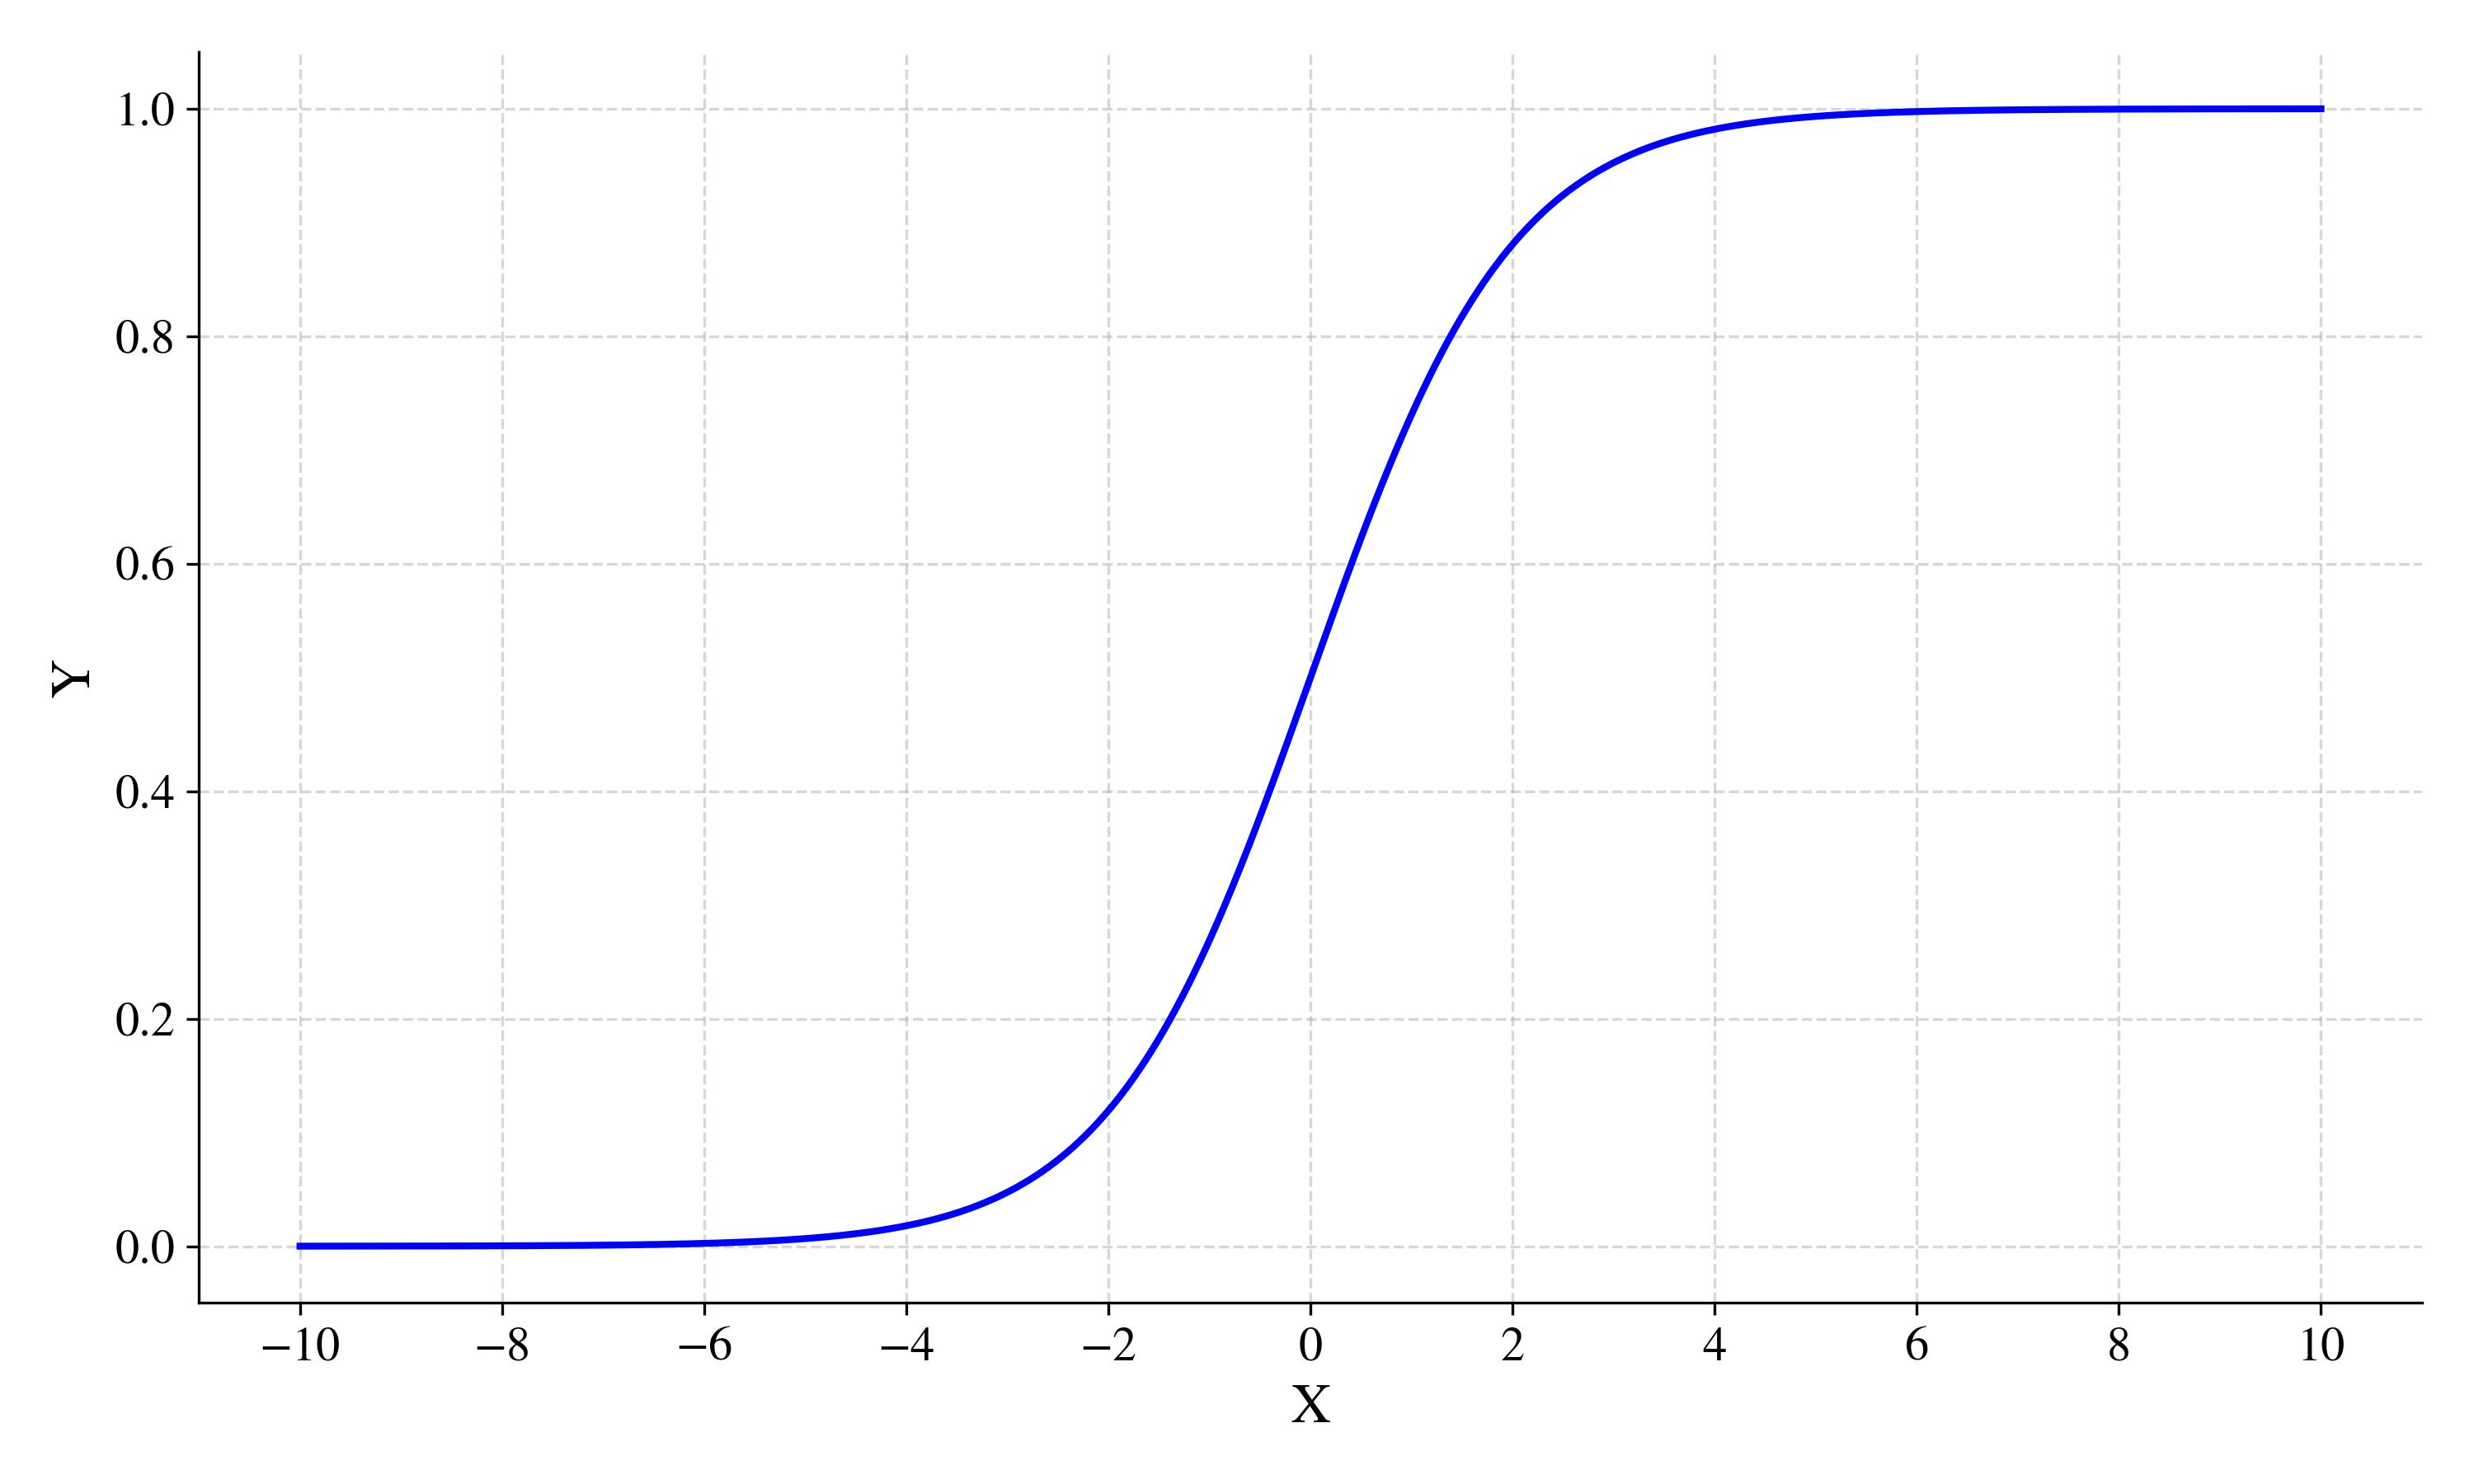
\includegraphics[width=130mm]{Figures/sigmoid.jpg}
    \centering{\begin{source}Author's simulation in Python\end{source}}\vspace{-1em}
\end{figure}

The linear form of the logistic regression with $n$ features can be written as:
\begin{equation}\label{eq}
    \ln\left(\frac{P}{1-P}\right) = \beta_0  + \sum_{i=1}^{n} \beta_i X_i
\end{equation}

where $P$ is the probability of the occurred event, conditional on the set of given features. Let us denote $Y=1$ as an observed target instance where the event occurred (e.g., default), then:
\begin{equation}\label{eq}
    P = \operatorname{Pr}(Y=1 \mid X)
\end{equation}

Therefore, the term within the natural logarithm is the odds or more particularly, the ratio of the probability of the event with respect to the probability of non-event, both conditional on the same set of given features.
\begin{equation}\label{eq}
    \begin{aligned}
    \frac{P}{1-P}  {} & = \frac{\operatorname{Pr}(Y=1 \mid X_1,X_2,\ldots,X_n)}{1-\operatorname{Pr}(Y=1 \mid X_1,X_2,\ldots,X_n)} \\
    & = \frac{\operatorname{Pr}(Y=1 \mid X_1,X_2,\ldots,X_n)}{\operatorname{Pr}(Y=0 \mid X_1,X_2,\ldots,X_n)}
\end{aligned}
    \end{equation}

Referring to the previous equations, solving for $P$, henceforth we get a final equation for computing the probability of occurred event with usage of logistic regression:
\begin{equation}\label{eq}
P = \frac{1}{1+e^{-\left(\beta_0 + \displaystyle\sum_{i=1}^{n} \beta_i X_i\right)}}
\end{equation}

Regarding the loss function minimized when estimating the model's parameters, the logistic regression uses the cross-entropy loss function, also known as log loss.
This loss function is also used as an evaluation metric for the model's performance, which is further described in \autoref{subsubsec:logloss}.
Let us denote the loss function as $L(y, p)$, where $y$ is the actual target values and $p$ is the predicted probability scores. To this loss function, we can also additionally employ a regularization term $C$ in order to prevent overfitting \citep{pramoditha2021mitigate} by penalizing the coefficients' magnitudes.
We distinguish 3 types of regularization (penalty) types:
\begin{itemize}\setlength\itemsep{0em}
    \item \textbf{L1} - Lasso regularization, which takes the absolute value of the coefficients' magnitudes.
\end{itemize}
\begin{equation}\label{eq:l1}
    L(y, p)_{L1}  = L(y, p) + C \sum_{j=1}^{k} \mid w_j \mid
\end{equation}
\begin{itemize}\setlength\itemsep{0em}
    \item \textbf{L2} - Ridge regularization, which squares the coefficients' magnitudes.
\end{itemize}
\begin{equation}\label{eq:l2}
    L(y, p)_{L2}  = L(y, p) + C \sum_{j=1}^{k} w_j^2
\end{equation}
\begin{itemize}\setlength\itemsep{0em}
    \item \textbf{Elastic Net} - Combination of L1 and L2 regularizations.
\end{itemize}
\begin{equation}\label{eq:elasticnet}
    L(y, p)_{ElasticNet} = L(y, p) + C \sum_{j=1}^{k} \left[ \alpha \mid w_j \mid + (1-\alpha) w_j^2 \right]
\end{equation}
where $\alpha$ indicates the weight of $L1$ penalty in the $ElasticNet$ penalty.

\subsection{Decision Tree}
\label{subsec:dt}

Decision Tree is a rule--based algorithm which aims to partition the data into smaller and more homogeneous subsets. Such tree contains nodes, which are also visualized in \autoref{fig:dtnodes}, namely:
\begin{itemize}\setlength\itemsep{0em}
	\item \textbf{Root node} - the topmost node of the tree where the splitting begins.
	\item \textbf{Internal node} - the non--terminal nodes as a result of the split and can be further split into another subsets.
	\item \textbf{Leaf node} - the terminal nodes as a results of the split and cannot be further split into another subsets.
\end{itemize}
\begin{figure}[H]
    \centering
    \caption{Decision Tree's Nodes}\vspace{0.5em}
    \label{fig:dtnodes}\
    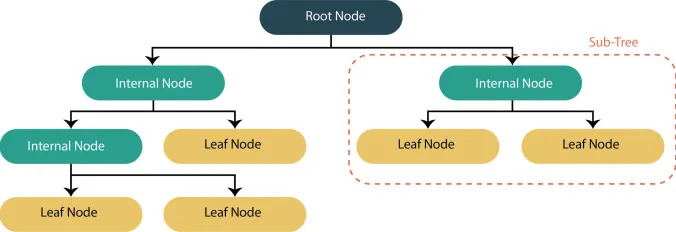
\includegraphics[width=130mm]{Figures/dtnodes.jpg}
    \centering{\begin{source}\citep{gauhar2020decision}\end{source}}\vspace{-1em}
\end{figure}

The splitting process is based on the homogeneity or so called purity of the node with respect to the target variable \citep{provost2013data}.
In other words, we want to have the node as pure as possible which means that the node should contain as high proportion of one class as possible.
In this case, the node should either contain high proportion of defaulters or non--defaulters, respectively.
Such splitting processs starts from the root node and continues until the leaf nodes are pure enough or until the stopping criteria are met.
The stopping criteria can be either a maximum depth of the tree, minimum number of observations within the node or minimum number of observations within the leaf node.
One way to measure impurity is using Entropy which ranges from 0 to 1 and is defined as:
\begin{equation}\label{eq}
    E = -\sum_{i=1}^{n} p_i \log_2 \left(p_i\right)
    \end{equation}
where $p_i$ is the probability of the occurrence of the event $i$, or in other words, it is a fraction of the observations belonging to the class $i$ within given node. In credit risk modelling terms, it is a proportion of defaulters within given node and $1-p_i$ is a proportion of non--defaulters within given sample.
The lower Entropy value, the purer the node is, i.e., the more homogeneous the subset is, where the frequency of one class is dominant to other class.
Therefore, the goal is to minimize the Entropy value since we want to have the purest nodes as possible, i.e., the nodes where is either a high proportion of defaulters or non--defaulters. 
However, the Entropy is not the only way to measure the impurity of the node. Another way is using Gini Impurity which ranges from 0 to 0.5 and is defined as:
\begin{equation}\label{eq}
    G = 1 - \sum_{i=1}^{n} p_{i}^{2}
\end{equation}
Both impurity measures are depicted in \autoref{fig:impurity} which we want to both of them minimize. Thus, we choose such feature and such rule which result in the lowest impurity measure. Such process is repeated until the stopping criteria are met or until the leaf nodes are pure enough.
\begin{figure}[H]
    \centering
    \caption{Gini Impurity vs. Entropy}\vspace{0.5em}
    \label{fig:impurity}\
    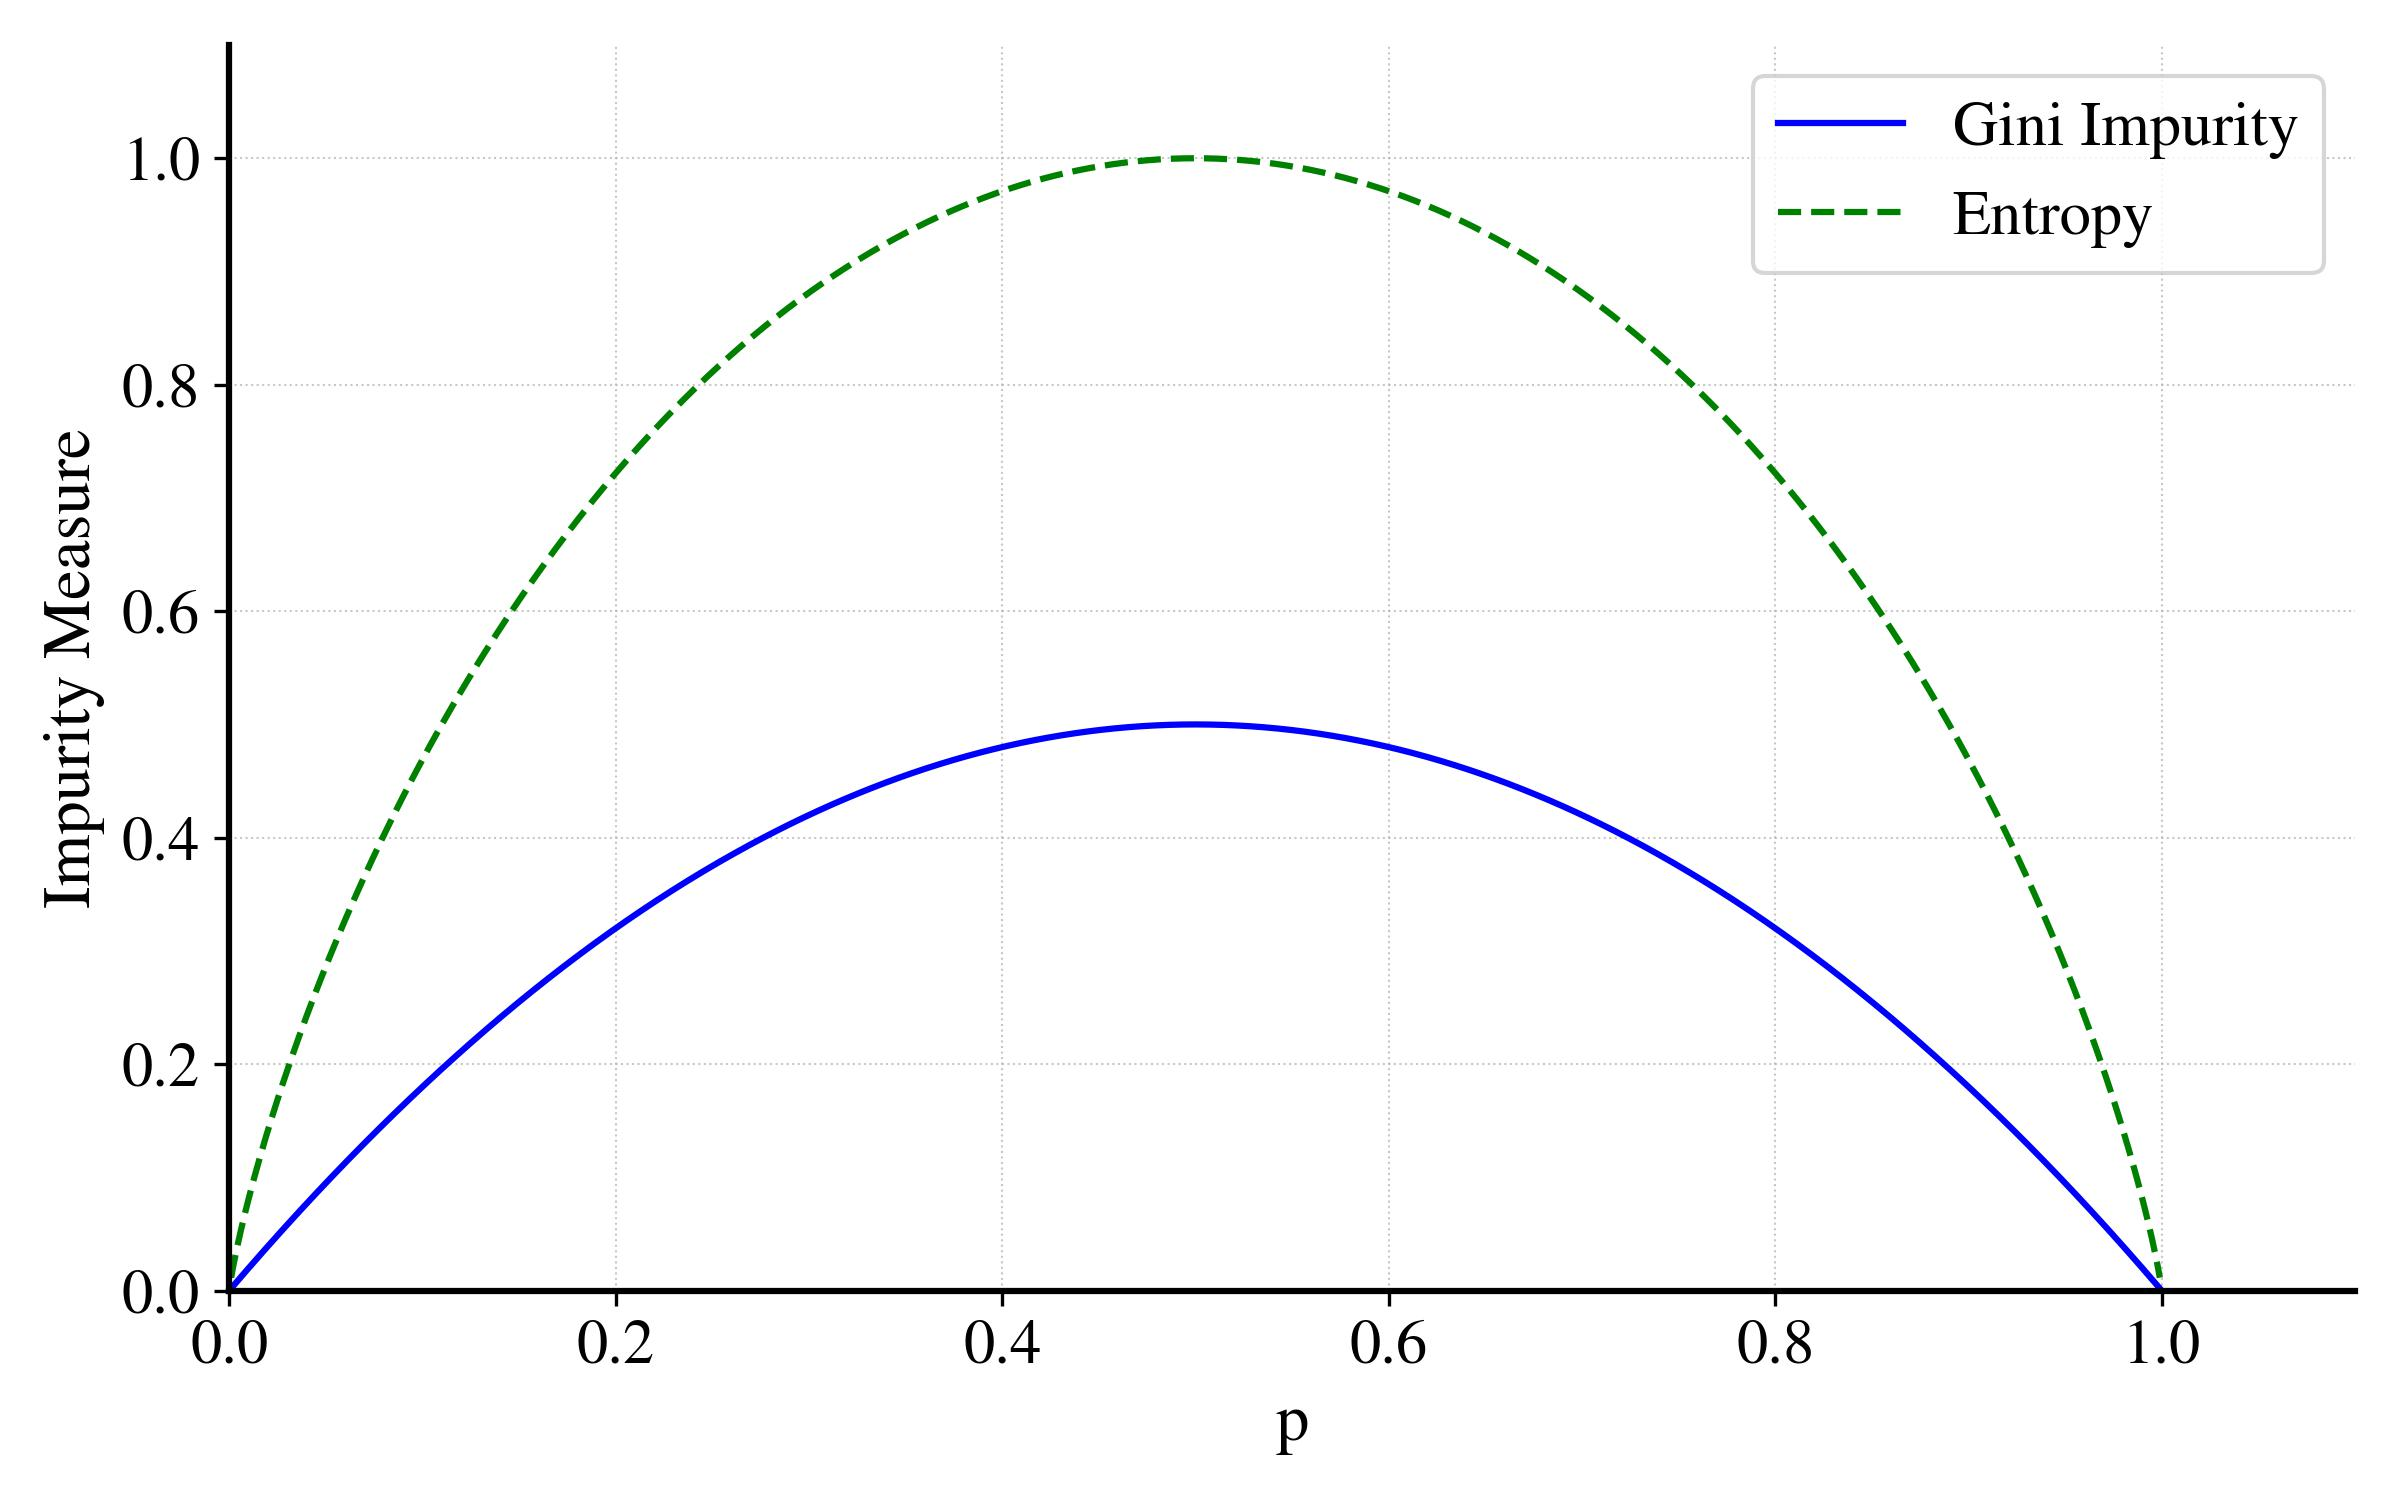
\includegraphics[width=130mm]{Figures/impurity.jpg}
    \centering{\begin{source}Author's simulation in Python\end{source}}\vspace{-1em}
\end{figure}

After the training, Decision Tree predicts the target variable based on the rules which are stored in the tree.
The prediction process starts from the root node and continues until the leaf node is reached. Within the leaf node, the prediction can be either the most frequent class within the node or the probability of the occurrence of the event, i.e., the proportion of defaulters within given node.

\subsection{Naive Bayes}

Naive Bayes is a classification and probabilistic machine learning algorithm which is based on Bayes theorem which is defined as:
\begin{equation}\label{eq}
    \operatorname{Pr}\left(C=c \mid E \right) = \frac{\operatorname{Pr}\left(C=c\right) \times \operatorname{Pr}\left(E \mid C=c\right)}{\operatorname{Pr}\left(E\right)}
\end{equation}

where:
\begin{itemize}\setlength\itemsep{0em}
	\item $\operatorname{Pr}\left(C=c \mid E \right)$ is the posterior probability which is the probability that the target variable $C$ takes on the class of interest $c$ after taking the evidence $E$.
	\item $\operatorname{Pr}\left(C=c\right)$  is the prior probability of the class $c$, i.e.,the probability we would assign to the class $c$ before seeing any evidence $E$.
	\item $\operatorname{Pr}\left(E \mid C=c\right)$ is the probability of seeing the evidence $E$ conditional on the given class $c$.
	\item $\operatorname{Pr}\left(E\right)$ is the probability of the evidence $E$.
\end{itemize}

With regards to the binary classification, we can substitute $Y$ as a target variable instead $C$, and set of features $X$ which will refer to the set of evidence $E$., henceforth the probability of $Y$ using the Naive Bayes algorithm can be mathematically expressed as:
\begin{equation}\label{eq}
    \operatorname{Pr}\left(Y \mid X \right) = \frac{\operatorname{Pr}\left(Y\right) \times \operatorname{Pr}\left(X \mid Y \right)}{\operatorname{Pr}\left(X\right)}
\end{equation}

One of the assumptions of this algorithm is the conditional probabilistic independence among the features.
Since all the $X$ features' values combinations do not have to appear at all, we assume their independence \citep{cichosz2014data}.
Therefore, instead of computing the probability of all features together, conditional on the class event, for each feature $X$ we compute the conditional joint probability of $X$ given the class event. Hence:
\begin{equation}\label{eq}
    \operatorname{Pr}\left(X  \mid Y \right) = \prod_{i=1}^{n} \operatorname{Pr}\left(X_i \mid Y\right)
\end{equation}

Furthermore, the second adjustment is applied to the denominator of the Bayes theorem, i.e., $\operatorname{Pr}\left(X\right)$ - since such probability is constant over all the values of the class event, we can omit it from the equation. Therefore, the posterior probability of the class event $Y$ conditional on the subset of features $X$ can be expressed as:
\begin{equation}\label{eq}
    \operatorname{Pr}\left(Y \mid X \right) = \prod_{i=1}^{n} \operatorname{Pr}\left(X_i \mid Y\right) \times \operatorname{Pr}\left(Y\right)
\end{equation}

During the training process, the Naive Bayes algorithm computes $\operatorname{Pr}\left(Y\right)$ and $ \operatorname{Pr}\left(X \mid Y \right)$ for each class event $Y$ and each feature $X$.
In terms of default status, it calculates the proportion of defaulters  $\operatorname{Pr}\left(Y = 1\right)$ and non--defaulters $\operatorname{Pr}\left(Y=0\right)$ within given training sample as well as the proportion of defaulters and non--defaulters within given feature $X$.


When it comes to the predictions or classification of new instances, we use the trained Naive Bayes model, i.e., the computed probabilities $\operatorname{Pr}\left(Y\right)$ and $ \operatorname{Pr}\left(X \mid Y \right)$ for both default and non--default class.
Specifically, based on the new instance's features $X$, we determine the computed $\operatorname{Pr}\left(Y\right)$ and $ \operatorname{Pr}\left(X \mid Y \right)$ for both classes and aftewards, as a predicted class, we choose such class with the highest posterior probability. In general, the prediction while maximizing posterior probability is given as:
\begin{equation}\label{eq:nb-corrected}
    \operatorname{Pr}\left(Y \mid X \right) = \operatorname{argmax}_{y \in Y} \operatorname{Pr}\left(X \mid Y = y\right) \times \operatorname{Pr}(Y = y)
\end{equation}
Specifically, in terms of binary classification for prediction of given class, whether it is default or non--default, we can compute the probability of the default event ($1$) and non--default event ($0$), and choose the class with the higher probability.
\begin{equation}\label{eq}
    \operatorname{Pr}\left(Y \mid X \right)  = \max \left(\operatorname{Pr}\left(Y=1 \mid X\right), \operatorname{Pr}\left(Y=0 \mid X\right)\right)
\end{equation}
where:
\begin{equation}
    \operatorname{Pr}\left(Y=0 \mid X \right) = \operatorname{Pr}\left(Y=0\right) \times \prod_{i=1}^{n} \operatorname{Pr}\left(X_i \mid Y=0\right)
\end{equation}
respectively:
\begin{equation}\label{eq:lastnbmax1}
    \operatorname{Pr}\left(Y=1 \mid X \right) = \operatorname{Pr}\left(Y=1\right) \times \prod_{i=1}^{n} \operatorname{Pr}\left(X_i \mid Y=1\right)
\end{equation}

This algorithm works well only if the features are categorical.
However, most of the data sets contain continuous features as well.
Therefore, we introduce \textbf{Gaussian Naive Bayes} algorithm which is suitable for continuous features. Such algorithm assumes that the features follow Normal (Gaussian) distribution, given the class label \citep{jahromi2017non}.
Assuming the class event $Y=1$, we can derive probability density function of particular value $x$ of the continuous feature $X$ as:
\begin{equation}\label{eq:lastgnb}
    \operatorname{Pr}\left(X = x \mid Y = 1\right) = \frac{1}{\sqrt{2 \pi \sigma_{X \mid Y=1}^{2}}} \exp \left(-\frac{\left(x - \mu_{X \mid Y=1}\right)^{2}}{2 \sigma_{X \mid Y=1}^{2}}\right)
\end{equation}
where $\mu_{X \mid Y=1}$ and $\sigma_{X \mid Y=1}$ is the mean and variance of $X$, respectively, given the the class event $Y=1$.
Afterwards, $\operatorname{Pr}\left(X = x \mid Y = 1\right)$ derived from the Gaussian distribution can be substituted into \autoref{eq:lastnbmax1}.
\subsection{K-Nearest Neighbors}
\label{subsec:knn-theory}

The goal of K-nearest Neighbors algorithm (henceforth KNN) is to find $k$ instances that are most similar to particular instances $y$ in the $n$--dimensional space, where $n$ is the number of features.
The principle of this algorithm consists in the similarity between the instances as it assumes that the similar instances are close to each other.
Based on the predetermined $k$ neighbors, it will predict the class based on the $k$ nearest instances.


There are several ways how to measure the distance. The most used one is the Euclidean distance. Geometrically, it is a straight line between the two points  and within two-dimensional space, it can be derived from the Pythagorean theorem, where the hypotenuse is the straight line measuring the distance. In the $n$-dimensional space, we take the sum the squared differences between the data points $x$ and $y$, underneath the square root in order to compute the total Euclidean distance.
\begin{equation}\label{eq}
d_{Euclidean}(x,y) = \sqrt{\sum\limits_{i=1}^{n} (x_i - y_i)^2}
\end{equation}

Other distance measure is the Manhattan distance measure, which is known as a city block distance, referring to the real-life problems, more particularly in order to reach particular destination, we have to take the path in between the blocks.
Mathematically, it is similar to the Euclidean distance, but instead of squared differences, it sums the absolute differences between the data points.
\begin{equation}\label{eq}
d_{Manhattan}(x,y) = \sqrt{\sum\limits_{i=1}^{n} |x_i - y_i|}
\end{equation}

The last measure is the Minkowski distance which is the generalized form Euclidean or Manhattan distance respectively.
It depends on $p$ which represents the order of the norm. Hence, the Euclidean distance has the second order of the norm, whereas Manhattan distance has the first order of the norm.
\begin{equation}\label{eq}
d_{Minkowski}(x,y) = \sqrt[p]{\sum\limits_{i=1}^{n} |x_i - y_i|^p}
\end{equation}

Within the training process, KNN memorizes training instances and afterwards when it encounters a new instance, it tries to search for such training instance(s) which most strongly resembles the new instance \citep{witten2011data}.
Therefore, After the training process, when it comes to the prediction, the KNN compares the new instance to the training instances, calculates the distances between the the new input and the training instances, and predicts the class based on on the majority voting within the $k$ nearest neighbors, or predicts the probability score as the fraction of positive instances within the $k$ nearest neighbors.


In the following \autoref{fig:knn-example}, let us consider 2--dimensional space and that $k$ is equal to 4, hence we are looking at four nearest neighbors for such new instance. Further, let us consider two classes - red squares and green triangles.
By looking at the four nearest neighbors, we can observe that three out of the four nearest neighbors are the red triangles.
Therefore, when applying majority voting, KNN would predict such instance as a red triangle, or would predict a probability score of 0.75 for the red triangle.

\begin{figure}[H]
    \centering
    \caption{K-Nearest Neighbors with $k=4$}\vspace{0.5em}
    \label{fig:knn-example}\
    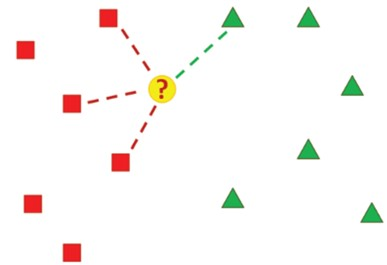
\includegraphics[width=70mm]{Figures/KNN_example.jpg}

    \centering{\begin{source}\citep{mucherino2009data}\end{source}}\vspace{-1em}
\end{figure}
\subsection{Random Forest}

Random forest is an ensemble algorithm which is a collection of decision trees where each tree is independently trained on on a bootstrap sample of the training data \citep{han2011data}, i.e., on a on a set which is randomly sampled from the training data with replacement and which has the same size as the training data. In such way, each bootstrap sample is unique and can contain duplicates of the original data or does not have to contain all the original data.
Another aspect of randomness in such algorithm, particularly in the variability within trees, is the number of features considered for the split at each node.
Instead of considering all the features of the length $M$, it randomly selects a subset of features of the length $m$ (where $m<M$) and chooses the best split from the subset.
The training process of individual decision tree is the same as described in \autoref{subsec:dt}.

Within classifying new instances, the random forest algorithm predicts the class based on the majority voting of the individual decision trees or predicts a probability as an average of the probabilities of the individual decision trees \citep{randomforestmalley}, thus:
\begin{equation}
    \operatorname{Pr}\left(Y=1 \mid X \right) = \frac{1}{B} \sum_{b=1}^{B} \operatorname{Pr}\left(Y=1 \mid X, T_b \right)
\end{equation}
where $B$ is the number of trees and $T_b$ is the $b$-th tree. Such algoritm is depicted on the \autoref{fig:rf-example} for the visual representation.
\begin{figure}[H]
    \centering
    \caption{Random Forest Diagram}\vspace{0.5em}
    \label{fig:rf-example}\
    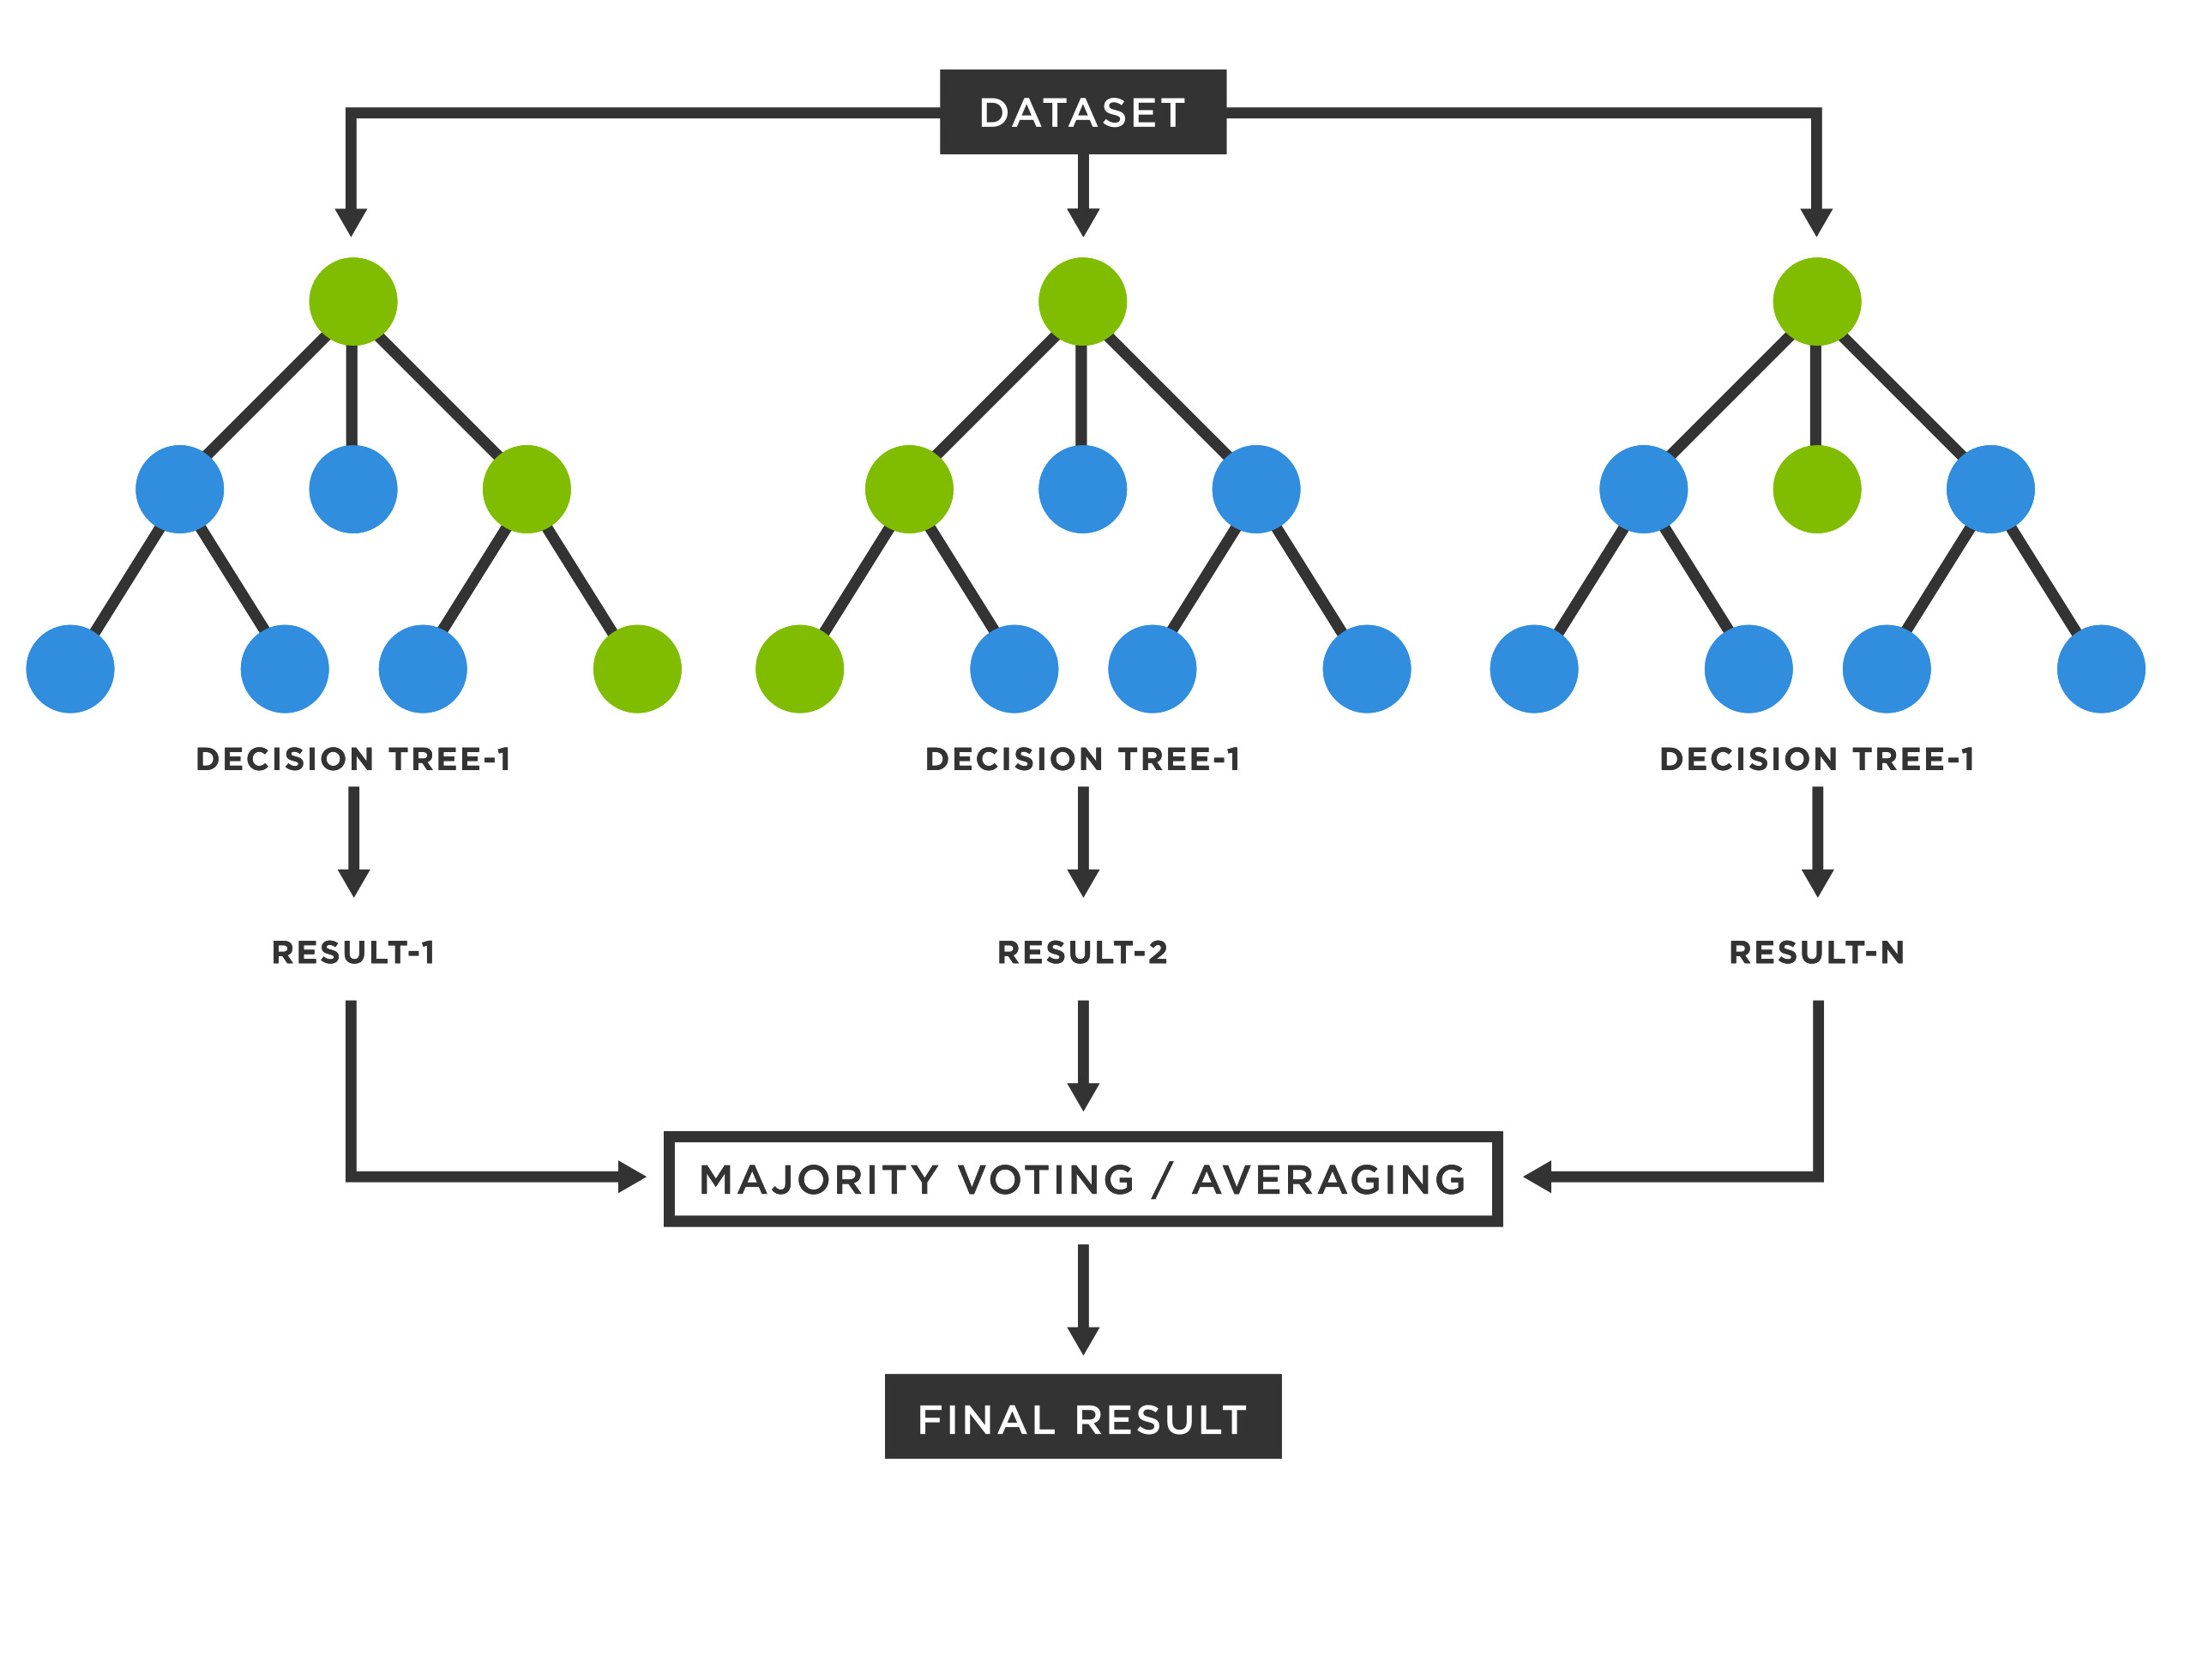
\includegraphics[width=120mm]{Figures/random-forest-diagram.jpg}

    \centering{\begin{source}\citep{TIBCO2023}\end{source}}\vspace{-1em}
\end{figure}
\subsection{Gradient Boosting}
In contrast to Random Forest whose trees are trained independently, i.e., in a parallel way, Gradient Boosting trains trees are trained in a sequential way, where each tree is trained on the residuals of the previous tree \citep{ayyadevara2018pro}, as a sequential building series of dependent weak learners, i.e., decision trees, in order to create a strong learner.

According to Dias \citep{dias2018comparison}, before adding any weak learners, first we need to initialize a model $F_0(x)$ which is a constant value computed by minimizing the sum of the loss function $L$ over all training samples, i.e., we look for such $\gamma$ constant which minimizes the loss function $L$, hence:
\begin{equation}
    F_{0}(x) = \arg \min _{\gamma} \sum_{i=1}^{n} L\left(y_{i}, \gamma\right)
\end{equation}
Then, for $m \in M$, where $M$ is the total number of iterations or the number of tree estimators:
\begin{itemize}\setlength\itemsep{0em}
    \item[1.] Compute pseudo--reisduals for each training sample pair $(x_i, y_i)$ as the negative gradient of the loss function $L$ with respect to the the prediction $F_{m-1}(x)$ of the previous model $F_{m-1}(x)$, hence:
\end{itemize}
\begin{equation}
    r_{i,m} = -\left[\frac{\partial L\left(y_{i}, F\left(x_{i}\right)\right)}{\partial F\left(x_{i}\right)}\right]_{F(x)=F_{m-1}(x)}
\end{equation}
\begin{itemize}\setlength\itemsep{0em}
    \item[2.] Train a weak learner $h_m(x)$ with the training data as features and the pseudo--residuals as the target values $(x_i, r_{i,m})$, and then compute the learning rate $\gamma_m$ which minimizes the loss function $L$ when adding the weak learner $h_m(x)$ to the previous model $F_{m-1}(x)$, hence:
\end{itemize}
\begin{equation}
    \gamma_{m} = \arg \min _{\gamma} \sum_{i=1}^{n} L\left(y_{i}, F_{m-1}\left(x_{i}\right)+\gamma h\left(x_{i}\right)\right)
\end{equation}
\begin{itemize}\setlength\itemsep{0em}
    \item[3.] Update the model $F_m(x)$ by adding the weak learner $h_m(x)$ with the learning rate $\gamma_m$, hence:
\end{itemize}
\begin{equation}
    F_m(x) = F_{m-1}(x) + \gamma_m h(x)
\end{equation}
Afterwards, such algorithm outputs the final model $F_M(x)$ as a combination of the initial model and the $M$ weak learners.

\subsection{Support Vector Machine}

Support Vector Machine (henceforth SVM) is machine learning algorithm which can handle both linear and non--linear classification problems and tries to transform original training data into a higher dimension, where the class points are linearly separable by a (linear) decision boundary, also known as hyperplane \citep{han2011data}.
In particular, SVM tries to maximize the margin which is the distance between the separating hyperplane and the support vectors, i.e., the training data points which are equally closest and parallel to such hyperplane \citep{tatsat2020machine}, as shown in \autoref{fig:svm-example}.

\begin{figure}[H]
    \centering
    \caption{Support Vector Machine 2D Hyperplane}\vspace{0.5em}
    \label{fig:svm-example}\
    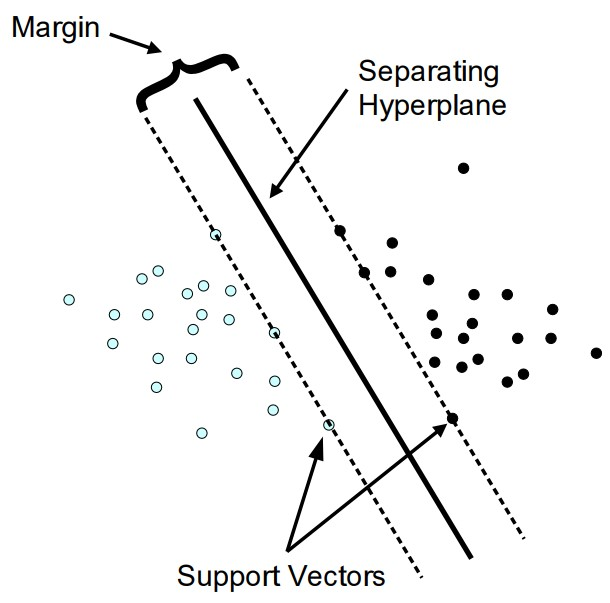
\includegraphics[width=60mm]{Figures/svmhyperplane.jpg}

    \centering{\begin{source}\citep{meyer2015support}\end{source}}\vspace{-1em}
\end{figure}

The hyperplane can be expressed as follows, where $X$ are the features data, $W$ is the vector of the weights and $b$ is the intercept:
\begin{equation}\label{eq:wxdo0}
    W \cdot X + b = 0
\end{equation}
Thus, the data points which lie above the hyperplane are classified as 1 and otherwise \citep{hsu2002comparison}.
Moreover, the distance between the hyperplane and any training data point is expressed as $\frac{1}{\|W\|}$, where $\|W\|$ is Euclidean the norm of the weight vector $W$.
In order to maximize the margin, we maximize following term as we want to maximize both sides of below and above the hyperplane, therefore:
\begin{equation}
    \min {\frac{2}{\|W\|}}
\end{equation}
When the data are not linearly separable, SVM transforms the original data points into a higher dimensional space using non--linear mapping function, also known as kernel \citep{han2011data}.
In general, kernel function for the training tuples $(X_i,X_j)$ can be expressed as:
\begin{equation}
    K(X_i,X_j) = \phi(X_i) \cdot \phi(X_j)
\end{equation}
where $\phi$ is mapping function for high--dimensional projection of the feature space. According to Patle \citep{patle2013svm}, the most common kernel functions. where $\gamma$ and $r$ and $d$ represent the kernel parameters, are:
\begin{itemize}\setlength\itemsep{0em}
    \item $d$--degree polynomial kernel:
\end{itemize}
\begin{equation}
    K\left(X_i,X_j\right) = (1+X_i \cdot X_k)^{d}
\end{equation}
\begin{itemize}\setlength\itemsep{0em}
    \item Gaussian radial basis kernel:
\end{itemize}
\begin{equation}
    K(X_i,X_j) = \exp\left(-\gamma \|X_i-X_j\|^{2}\right)
\end{equation}
\begin{itemize}\setlength\itemsep{0em}
    \item Sigmoid kernel:
\end{itemize}
\begin{equation}
    K(X_i,X_j) = \tanh(\gamma X_i \cdot X_j + r)
\end{equation}
In some cases, the data cannot be linearly separable in higher dimensional space, i.e., we need to account for some potential errors, thus we introduce regularization factor $C$  for penalizing the errors $\xi$.
Therefore, in order to maximize the margin as well as to allow for errors, we minize the following term:
\begin{equation}
    \min \frac{1}{2} \|W\| + C \sum_{i=1}^{N} \xi
\end{equation}
Hence, by minimizing $\frac{1}{2} \|W\|$ we minimize the weights (i.e, maximize the margin), by minimizing $\xi$ we reduce the number of training error, and by tuning $C$ we balance between these two properties \citep{hsu2002comparison}. 

Note, that SVM does not predict probability scores by default, but rather predicted classes based on the location whether the given data points are above or below the hyperplane.
In order to obtain SVM's probabilities. as stated by Lin \citep{lin2007note}, the Platt scaling \citep{platt1999probabilistic} can be applied as a surrogate model to estimate probability outputs. Particularly, it fits a logistic regression model with true labels as target variable and predictions produced by SVM as features to predict the probability scores.
Hence:
\begin{equation}
    \operatorname{Pr}\left(Y | f(x) \right) = \frac{1}{1 + \exp\left(A \cdot f(x) + B \right)} 
\end{equation}
where, $A$ and $B$ are the coefficients of the logistic regression model.

\subsection{Neural Network}
\label{subssec:nn}
Neural Network is a black--box machine learning algorithm which can handle very complex and non--linear relationship between. It contains several layers where each layer has a certain number of units (neurons). In general, we distinguish 3 type of layers as also visualized in \autoref{fig:nn-example}:
\begin{itemize}\setlength\itemsep{0em}
    \item \textbf{Input layer} - The initial layer wghich contains $n$ units, where $n$ is the number of features within the data set.
    \item \textbf{Output layer} - The final final layer which contains $m$ units, where $m$ is the number of classes within the target variable. Since we assume only binary classification algorithms, therefore the output layer contains only one unit.
    \item \textbf{Hiden layer} - The intermediate layer which is always between the two layers - either between the input and output layer or even between other hidden layers.
    \end{itemize}

\begin{figure}[H]
    \centering
    \caption{Neural Network Architecture}\vspace{0.5em}
    \label{fig:nn-example}\
    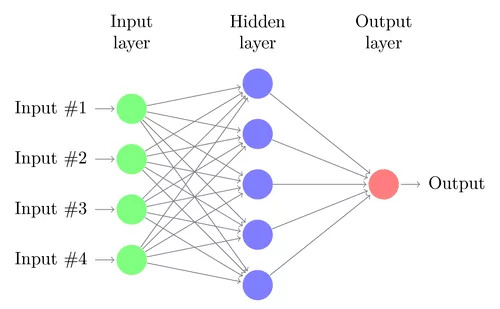
\includegraphics[width=100mm]{Figures/nn-example.jpg}

    \centering{\begin{source}\citep{Dilmegani2017}\end{source}}\vspace{-1em}
\end{figure}

The most common type of hidden layer is the fully connected layer where each unit is connected to each unit of the previous layer and to each unit in the next layer.
Thus, each unit receives the inputs from the previous layer, performs the computation and feed the output to the next layer - such process is called \textit{feed--forward}, hence feed--forward neural networks \citep{charu2018neural}.
Within the receiving the inputs, let us assume an integration function $g$ which performs a linear combination of the inputs $x$ and the weights $w$, and adds a bias term $b$.
Therefore, the output value $z$ of the single unit in hidden layer is calculated as:
\begin{equation}
    z = g\left(X,w\right)= b + \sum_{m=1}^{M} w_m x_m
\end{equation}
where $M$ indicates the number of units in the previous layer.
Before the output value $z$ is passed to the next layer, it is transformed by an activation function $f$ which is usually a non--linear function. The most common non--linear activation functions are:
\begin{itemize}\setlength\itemsep{0cm}
\item \textbf{ReLU} - Rectified Linear Unit (henceforth ReLU) is half--linear function which is rectified from the negative values to zero. The ReLU function is defined as:
\end{itemize}
\begin{equation}
    f(z) = \max(0,z)
\end{equation}
\begin{itemize}\setlength\itemsep{0cm}
    \item \textbf{Tanh} - Hyperbolic tangent (henceforth Tanh) is another widely used non--linear activation function which reminds of the sigmoid function. The Tanh function is limited to the range between -1 and 1, and is defined as:
    \end{itemize}
\begin{equation}
    f(z) = \frac{e^z - e^{-z}}{e^z + e^{-z}}
\end{equation}
\begin{itemize}\setlength\itemsep{0cm}
    \item \textbf{Sigmoid} - The logistic function was already described in \autoref{subsubsec:logisticregression}. Such function is usually used in the last hidden layer before the output layer as it maps the output to the range between 0 and 1, i.e., the predicted probability for binary classification. In terms of $z$, the sigmoid function is defined as:
    \end{itemize}
\begin{equation}
    f(z) = \frac{1}{1+e^{-z}}
\end{equation}
The training of neural network is an iterative process, where within each iteration (also called as epoch), the neural network is fed with the input, pass through the (hidden) layers to the output. The output is then compared with the actual value and the error is calculated.
Here comes another property of neural network which is the back--propagation, which updates all the weights and biases starting from the last layer by a small amount until the error is minimized as much as possible \citep{ayyadevara2018pro}.
The error is then backpropagated through the network and the weights are updated. The process is repeated until the error is minimized.

\newpage
\section{Evaluation Metrics}

This section focuses on particular measures through which it is possible to determine a predictive power of model in terms of its performance.
The are many ways, how to evaluate the model's performance, therefore, only the most common ones and the most relevant are further described.
Note, since default prediction regards classification tasks, therefore regression's evaluation metrics are omitted.
If not stated otherwise, the higher metric measure, the better the model's performance is.
\subsection{Confusion Matrix and Derived Metrics}


Confusion matrix is a table which summarizes the classification model's performance with respect to the actual classes and predicted classes.
It is a square $n \times n$ matrix, where $n$ determines number of classes within the target variable.
Let us denote the confusion matrix as $C\left(f\right)$ for classification algorithm $f$. 
Its elements can be denoted as $c_{i,j}$ where $i$ and $j$ refer to the row and column indices, respectively, or more particularly, $i$ refers to the actual class and $j$ to the class predicted by the classifier $f$.
Each element of the confusion matrix refers to the number of instances corresponding to actual class $i$ and predicted class $j$ \citep{japkowicz2011evaluating}. For instance, the element $c_{2,1}$ would refer to the number of instances which have the actual class $2$ but have been classified as class $1$.
Mathematically, the confusion matrix can be written as following:

\begin{equation}\label{eq}
C = {c_{i,j} = \sum_{l=1}^{m}[(y_l=i) \land (f(x_l)=j)]}
\end{equation}

Or either in matrix form as:

\begin{equation}\label{eq}
    C_{i \times j} = \begin{bmatrix}
    c_{1,1} & c_{1,2} & \cdots & c_{1,j} \\
    c_{2,1} & c_{2,2} & \cdots & c_{2,j} \\
    \vdots & \vdots & \ddots & \vdots \\
    c_{i,1} & c_{i,2} & \cdots & c_{i,j} \\
    \end{bmatrix}
\end{equation}

From the given matrix, the diagonal elements represent the numbers of correctly classified instances, whereas the non-diagonal elements represent the numbers of misclassified instances.
Further, let us consider a binary classification - hence, the confusion matrix will have a form of $2\times 2$:

\begin{equation}
    C_{2 \times 2} = \begin{bmatrix}
    c_{1,1} & c_{1,2} \\
    c_{2,1} & c_{2,2} \\
    \end{bmatrix}
\end{equation}


We can this rewrite confusion matrix, assuming 2 target variable classes $Positive$ and $Negative$, as:

\begin{equation}
    C_{2 \times 2} = \begin{bmatrix}
    TP & FN \\
    FP & TN \\
    \end{bmatrix}
\end{equation}

where:
\begin{itemize}\setlength\itemsep{0em}
    \item TP is the True Positive which refers to the number of instances which corresponds to the actual (\textit{True}) class $Positive$ and indeed have been correctly classified as class $Positive$.
	\item $FP$ is the False Positive which refers to the number of instances which corresponds to the actual (\textit{True}) class $Negative$, but have been incorrectly classified as class $Positive$. In the statistics and hypothesis--testing terms, it can be also called as Type 1 Error.
	\item $FN$ is the False Negative which refers to the number of instances which corresponds to the actual class $Negative$, but have been incorrectly classified as class $Positive$. In the statistics and hypothesis--testing terms, it can be also called as Type 2 Error.
	\item $TN$ is the True Negative which refers to the number of instances which corresponds to the actual class $Negative$ and indeed have been correctly classified as class $Negative$.
\end{itemize}

From such confusion matrix, we can derive several metrics which are further described on the following pages:

\subsubsection{Accuracy}
Such metric ranges from 0 to 1 and it describes in relatives terms how many instances the model has correctly predicted. Thus, the goal is to minimize the number of False Positives and False Negatives, or in credit risk modelling terms, number of defaulters which the model has classified as non--defaulters and number of non--defaulters which the model has classified as defaulters.
However, Accuracy is inappropriate metric for evaluation when having imbalanced class, i.e., where the distribution of the target variable is skewed.
In such case, the model can achieve a relatively high Accuracy even though it is not able to predict the minority class correctly \citep{brownlee2021failure}, thus it would lead to the misleading results.
This is the case of the credit risk modelling, when the loan portfolio oftenly have a lot of non--defaults and few defaults.
Therefore, it is deemed appropriate to consider other metrics when having imbalanced class.
\begin{equation}\label{eq}
    Accuracy = \frac{TP + FN}{TP + TN + FP + FN}
\end{equation}

\subsubsection{Recall}
\label{subsubsec:recall}
Such metric is also known as True Positive Rate (TPR) or Sensitivity, which also ranges from 0 to 1, and it describes in relative terms how many actual $Positive$ instances the model has correctly predicted out of all the actual $Positive$ instances. Thus, the goal is to minimize the number of False Negatives, i.e., number of defaulters which the model has classified as non--defaulters.
A lower value of recall could therefore indicates that either the model is not able to predict correctly the $True$ classes resulting in low number of True Positives and/or high number of False Negatives.
Recall metris is useful when having imbalanced class and should be used instead of accuracy metric as it measures the model's ability to correctly identify instances of the minority class (i.e., defaults).
Mathematically based on the confusion matrix elements, it can be computed as:
\begin{equation}\label{eq}
    Recall = \frac{TP}{TP + FN}
\end{equation}

\subsubsection{Precision}
This metric describes in relative terms how many predicted $Positive$ instances are actually $Positive$ out of all the predicted $Positive$ instances. Thus, the goal is to minimize the number of False Positives, i.e., number of non--defaulters which the model has classified as defaulters.
A lower value of precision could therefore indicates that either the model is not able to predict correctly the $True$ classes (low number of True Positives) or its prediction of $True$ classes is noisy (high number of False Positives).
Precision is another metric which should be used instead of Accuracy when having imbalanced class as it tt measures the model's ability to correctly identify instances of the minority class while minimizing false positives (i.e., non--default instances which the model has classified as default).
Similarly, Precision also ranges from 0 to 1 and can be derived from the confusion matrix as follows:
\begin{equation}\label{eq}
    Precision = \frac{TP}{TP + FP}
\end{equation}
\subsubsection{F1 Score}
F1 score incorporates both Recall and Precision into a single value and takes on values between 0 and 1 as well.
Is it defined as a weighted harmonic mean of these two metrics \citep{brabec2020model} (where both Recall and Precision have uniform weights), and the goal is to minimize False Positives and False Negatives at the same time as within Accuracy.
Nevertheless, F1 score is deemed as more appropriate metric when dealing with imbalanced class as it provides more balanced evaluation of model's performance in imbalanced data sets compared to Accuracy.
\begin{equation}\label{eq}
    F1 = \frac{2 \times Precision \times Recall}{Precision + Recall} = \frac{2 \times TP}{2 \times TP + FP + FN}
\end{equation}

\subsubsection{Matthews Correlation Coefficient}
The drawback of Recall, Precision and F1 score is they are asymmetric measures, i.e., they do not take into account the True Negatives.
Therefore, such metrics' values will differ if we swap the positive and negative classes \citep{chicco2020advantages}, e.g., class 1 would indicate non--default and vice versa.
In order to overcome such drawback, Matthews Correlation Coefficient can be used as it is symmetric and it takes into account all the four elements of the confusion matrix as well as it captures imbalanced class issue.
Methodologically, Matthews Correlation Coefficient is defined as a discretization of Pearson correlation for the case of binary variables \citep{boughorbel2017optimal}.
Pearson correlation coefficient is defined as:
\begin{equation}\label{eq}
    r(x,y) = \frac{\sum\limits_{i=1}^n (x_i - \bar{x})(y_i - \bar{y})}{\sqrt{\sum\limits_{i=1}^n (x_i - \bar{x})^2} \sqrt{\sum\limits_{i=1}^n (y_i - \bar{y})^2}}
\end{equation}
Thus, assuming that $x$ is the vector of True labels and $y$ is the vector of predictions, the Matthews Correlation Coefficient can be defined as:
\begin{equation}\label{eq}
    MCC = \frac{TP \times TN - FP \times FN}{\sqrt{(TP + FP) (TP + FN) (TN + FP) (TN + FN)}}
\end{equation}
Matthews correlation coefficient ranges from -1 to 1, where 1 indicates perfect model's predictions, -1 indicates that model misclassifies all the instances and 0 indicates that model's predictions are not better than random guessing.
\subsection{ROC Curve and AUC}
\subsubsection{ROC Curve}
In order to derive Area Under the Curve (henceforth AUC), first we need to define Receiver Operating Characteristics (henceforth ROC) curve.
ROC curve is two-dimensional visualization of the model performance and shows trade--off beteen True Positive Rate ($TPR$) and False Positive Rate ($FPR$) based on varying the given threshold \citep{han2011data}. The former metric was already described in \autoref{subsubsec:recall}, the latter refers to the ratio of the number of $Negative$ instances which are classified as $Positive$ to the total number of the actual $Negative$ instances, hence:
\begin{equation}\label{eq}
    FPR = \frac{FP}{TN + FP}
\end{equation}

In order to construct ROC curve, we need to sort the instances by the predicted probability scores and based on the given probability score, we set a threshold - what will be above the threshold will be classified as $True$ instance and what is below the threshold will be classified as $False$ instance. Thus, each probability score threshold produces a differnt confusion matrix and hence, different $TPR$ and $FPR$ values \citep{fawcett2006introduction}.
Thus, if the probability is 1, the threshold will be 1 as well and hence:
\begin{itemize}\setlength\itemsep{0em}
    \item $TPR$ will be 0 because there is no probability which is higher than 1 and hence, everything will be classified as $Negative$ which will result into $TP$ of 0, and subsequently into $TPR$ of 0 as well.
	\item $FPR$ will be 0, too - since everything will be classified as $Negative$, therefore $FP$ will be 0 which implies $FPR$ to be 0, too.
\end{itemize}
On the other hand, if the probability is 0, the threshold will be 0 as well and hence:
\begin{itemize}\setlength\itemsep{0em}
    \item $TPR$ will be 1 because there is no probability which is lower than 0 and hence, everything will be classified as $Positive$ which will result into $FN$ of 0, and subsequently into $TPR$ of 1.
	\item $FPR$ will be 1, too - since everything will be classified as $Positive$, therefore $TN$ will be 0 which implies $FPR$ to be 1.
\end{itemize}

Thus, based on each threshold, the $TPR$ and $FPR$ will be to coordinates for single point within the graph and based on such points, we can construct the ROC curve, which can be depicted in \autoref{fig:roccurvetheory}.
Note that the diagonal line represents a random model which randomly guesses the $Positive$ class half the time in such way, that $FPR$ and $TPR$ are the same, i.e., 0.5 \citep{fawcett2006introduction}.
Logically, a decent model should perform better than the random model, thus it the ROC curve should be above the diagonal line.
Intuitively, the best possible theoretical model would have $TPR$ of 1 and $FPR$ of 0, meaning that all the $True$ actual classes should be predicted as $True$ and all the $False$ actual classes should not be classified as $True$
 Within the ROC curve, the given curve reaches the left top corner which corresponds to the coordinates of $TPR$ and $FPR$.

 \begin{figure}[H]
    \centering
    \caption{ROC Curve}\vspace{0.5em}
    \label{fig:roccurvetheory}\
    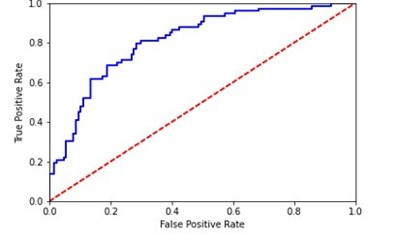
\includegraphics[width=100mm]{Figures/ROC_theory.jpg}

    \centering{\begin{source}Author's results in Python.\end{source}}\vspace{-1em}
\end{figure}
\subsubsection{AUC}

$AUC$ is basically the representation of ROC curve as a single number as it aggregates the performance on all possible thresholds ranging from 0 to 1.
$AUC$ can be interpreted as the probability that the randomly chosen actual $True$ instance is ranked higher than the randomly chosen actual $False$ instance \citep{janitza2013auc}.
As the $AUC$ is an area present underneath the ROC curve, mathematically, it can be computed with the definite integral where $x$ is the given threshold:
\begin{equation}\label{eq}
    AUC = \int_{0}^{1} TPR \left(FPR^{-1}\left(x \right)\right) dx
\end{equation}


Since ROC curve is a probability curve, thus it is considering distribution curve of $TP$ and distribution curve of $TN$, separated by particular threshold - hence, $TP$ would have probability scores above the given thresholds, whereas $TN$ would have probability scores below the threshold.
If these curves do not overlap, meaning the model can perfectly distinguish between the $Positive$ and $Negative$ values, therefore the $AUC$ would be 1 and the ROC curve would reach the left top corner.
However, this idealistic situation does not occur in the practice at all, but rather the two distributions are overlapping since the misclassification of the classes takes the place.
The bigger overlap, the lower $AUC$ is.
If the distributions are completely overlapping, it implies the $AUC$ of 0.5, meaning that the model cannot distinguish between the $Positive$ and $Negative$ classes, which is the worst scenario.
On the other hand, if the distributions are totally opposite (meaning that the $TP$ instances would have probability scores below the given threshold, whereas the $TN$ instances would have probability scores above the given threshold), the $AUC$ would be 0 since the model is predicting the $Positive$ actual classes instead of $Negative$ and vice versa \citep{narkhede2018understanding}.



\subsection{Kolmogorov-Smirnov Distance}

The Kolmogorov-Smirnov (KS) Distance is non--parametric metric for assessing discriminant power of a model as it measures distance between the cumulative distribution functions (henceforth CDF) between two classes, and is quantified as a maximum vertical absolute difference between such two CDF's \citep{adeodato2016equivalence}.
In credit risk modelling terms, we can express KS as follows:
\begin{equation}\label{eq}
    \text{Kolmogorov Smirnov} = \max_{0 \le t \le 1} \left| F_D \left(t \right) - F_{ND} \left(t \right) \right|
\end{equation}
where $F_D$ and $F_{ND}$ are the cumulative distribution functions of default and non-default cases, respectively, and $t$ is the probability score threshold which ranges between 0 and 1. $F_D$ and $F_{ND}$ are defined as follows:
\begin{equation}\label{eq}
    F_D \left(t \right) = \frac{1}{M_D} \sum_{i=1}^{M_D} I \left[f(x_i) \le t \right]
\end{equation}
\begin{equation}\label{eq}
    F_{ND} \left(t \right) = \frac{1}{M_{ND}} \sum_{i=1}^{M_D} I \left[f(x_i) \le t \right]
\end{equation}
where $M_D$ and $M_{ND}$ refer to the number of default and non-default cases, respectively, and $I$ is the indicator function which is equal to 1 if the condition is true and 0 otherwise \citep{doumpos2019analytical}.
 
\subsection{Somer's D}

The Somers' D is a metric which is part of the Kendall family of ranking measures. Particularly, assuming X-Y pairs, a Kendall's $\tau_{a}$ is defined as:
\begin{equation}\label{eq}
    \tau\left(X,Y\right) = \text{E} \left[ \text{sign}(X_i - X_j) \text{sign} (Y_i - Y_j) \right]
\end{equation}
Equivalently, Kendall's $\tau_{a}$ can be defined as the difference between the probability that the two X-Y pairs are \textit{concordant} and the probability that they are \textit{discordant}. X-Y pair is concordant if the larger of the $X$ values is paired with with larger of the $Y$ values, i.e, $X_i < X_j$ and $Y_i < Y_j$.
In contrast, X-Y pair is discordant if the larger of $X$ values is associated with smaller of $Y$ values or vice versa, i.e, $X_i < X_j$ and $Y_i > Y_j$, or $X_i > X_j$ and $Y_i < Y_j$ \citep{newson2002parameters}.
Therefore, Somers' D can be defined as the difference between the two conditional probabilities of concordance and discordance, given that the two $X$ values are unequal \citep{newson2014interpretation} as follows:
\begin{equation}
    D\left(Y \mid X\right) = \frac{\tau\left(X,Y\right)}{\tau\left(X,X\right)}
\end{equation}
In case of a binary classification, $X$ values would represent \textit{True} labels and $Y$ values would represent predicted probability scores as rank vectors. Such metric ranges from -1 to +1 (likewise as Matthews correlation coefficient +1). Thus, the higher value of Somers' D, the model's better ability to distinguish between borrowers who are likely to default and those who are not.

\subsection{Brier Score Loss}
Methodologically, Brier Score Loss is calculated in the same way as Mean Squared Error (henceforth MSE). However, Brier Score Loss is applied to the predicted probabilities (i.e., assumes that the target variable is dichotomous) \citep{comotto2022evaluation}, whereas MSE is rather used in regression tasks where is no assumption regarding the continuous target variable.
Henceforth, Brier Score Loss is defined as a mean squared error between the $True$ labels ($y$) and the predicted probabilities ($\hat{y}$) as follows:
\begin{equation}\label{eq}
    \text{Brier Score Loss} = \frac{1}{n} \sum_{i=1}^{n} (y_i - \hat{y}_i)^2
\end{equation}
Brier Score Loss ranges from 0 to 1, where the the ideal scenario would be Brier Score Loss of 0 - in such case, the model would be perfect predictive power.
\subsection{Log Loss}
\label{subsubsec:logloss}

Log loss, also know as logistic loss or cross--entropy loss, is a loss function metric which takes \textit{True} labels and predicted probabilities as an input and the minimize the difference between these two in a logarithmic function's form. Particularly, it indicates how close the predicted probabilities are to the corresponding $True$ labels. The more predicted probabilities diverges from the actual value, the more the log loss function penalizes the model's performance \citep{dembla2020intuition}.
\begin{equation}\label{eq}
    \text{Log Loss}  = -\frac{1}{N} \sum_{i=1}^{N} y_i \ln(p_i) + (1-y_i)\ln(1-p_i)
\end{equation}


Logically, the lower Log loss value, the better performance of the model is. As depicted in \autoref{fig:logloss}, we can observe the closer the predicted probability is closer to 1 with respect to the actual target class being equal to 1, the more is the log loss function closer to 0 which is desired in terms of model's performance.
\begin{figure}[H]
    \centering
    \caption{Log Loss Function for $Y=1$}\vspace{0.5em}
    \label{fig:logloss}\
    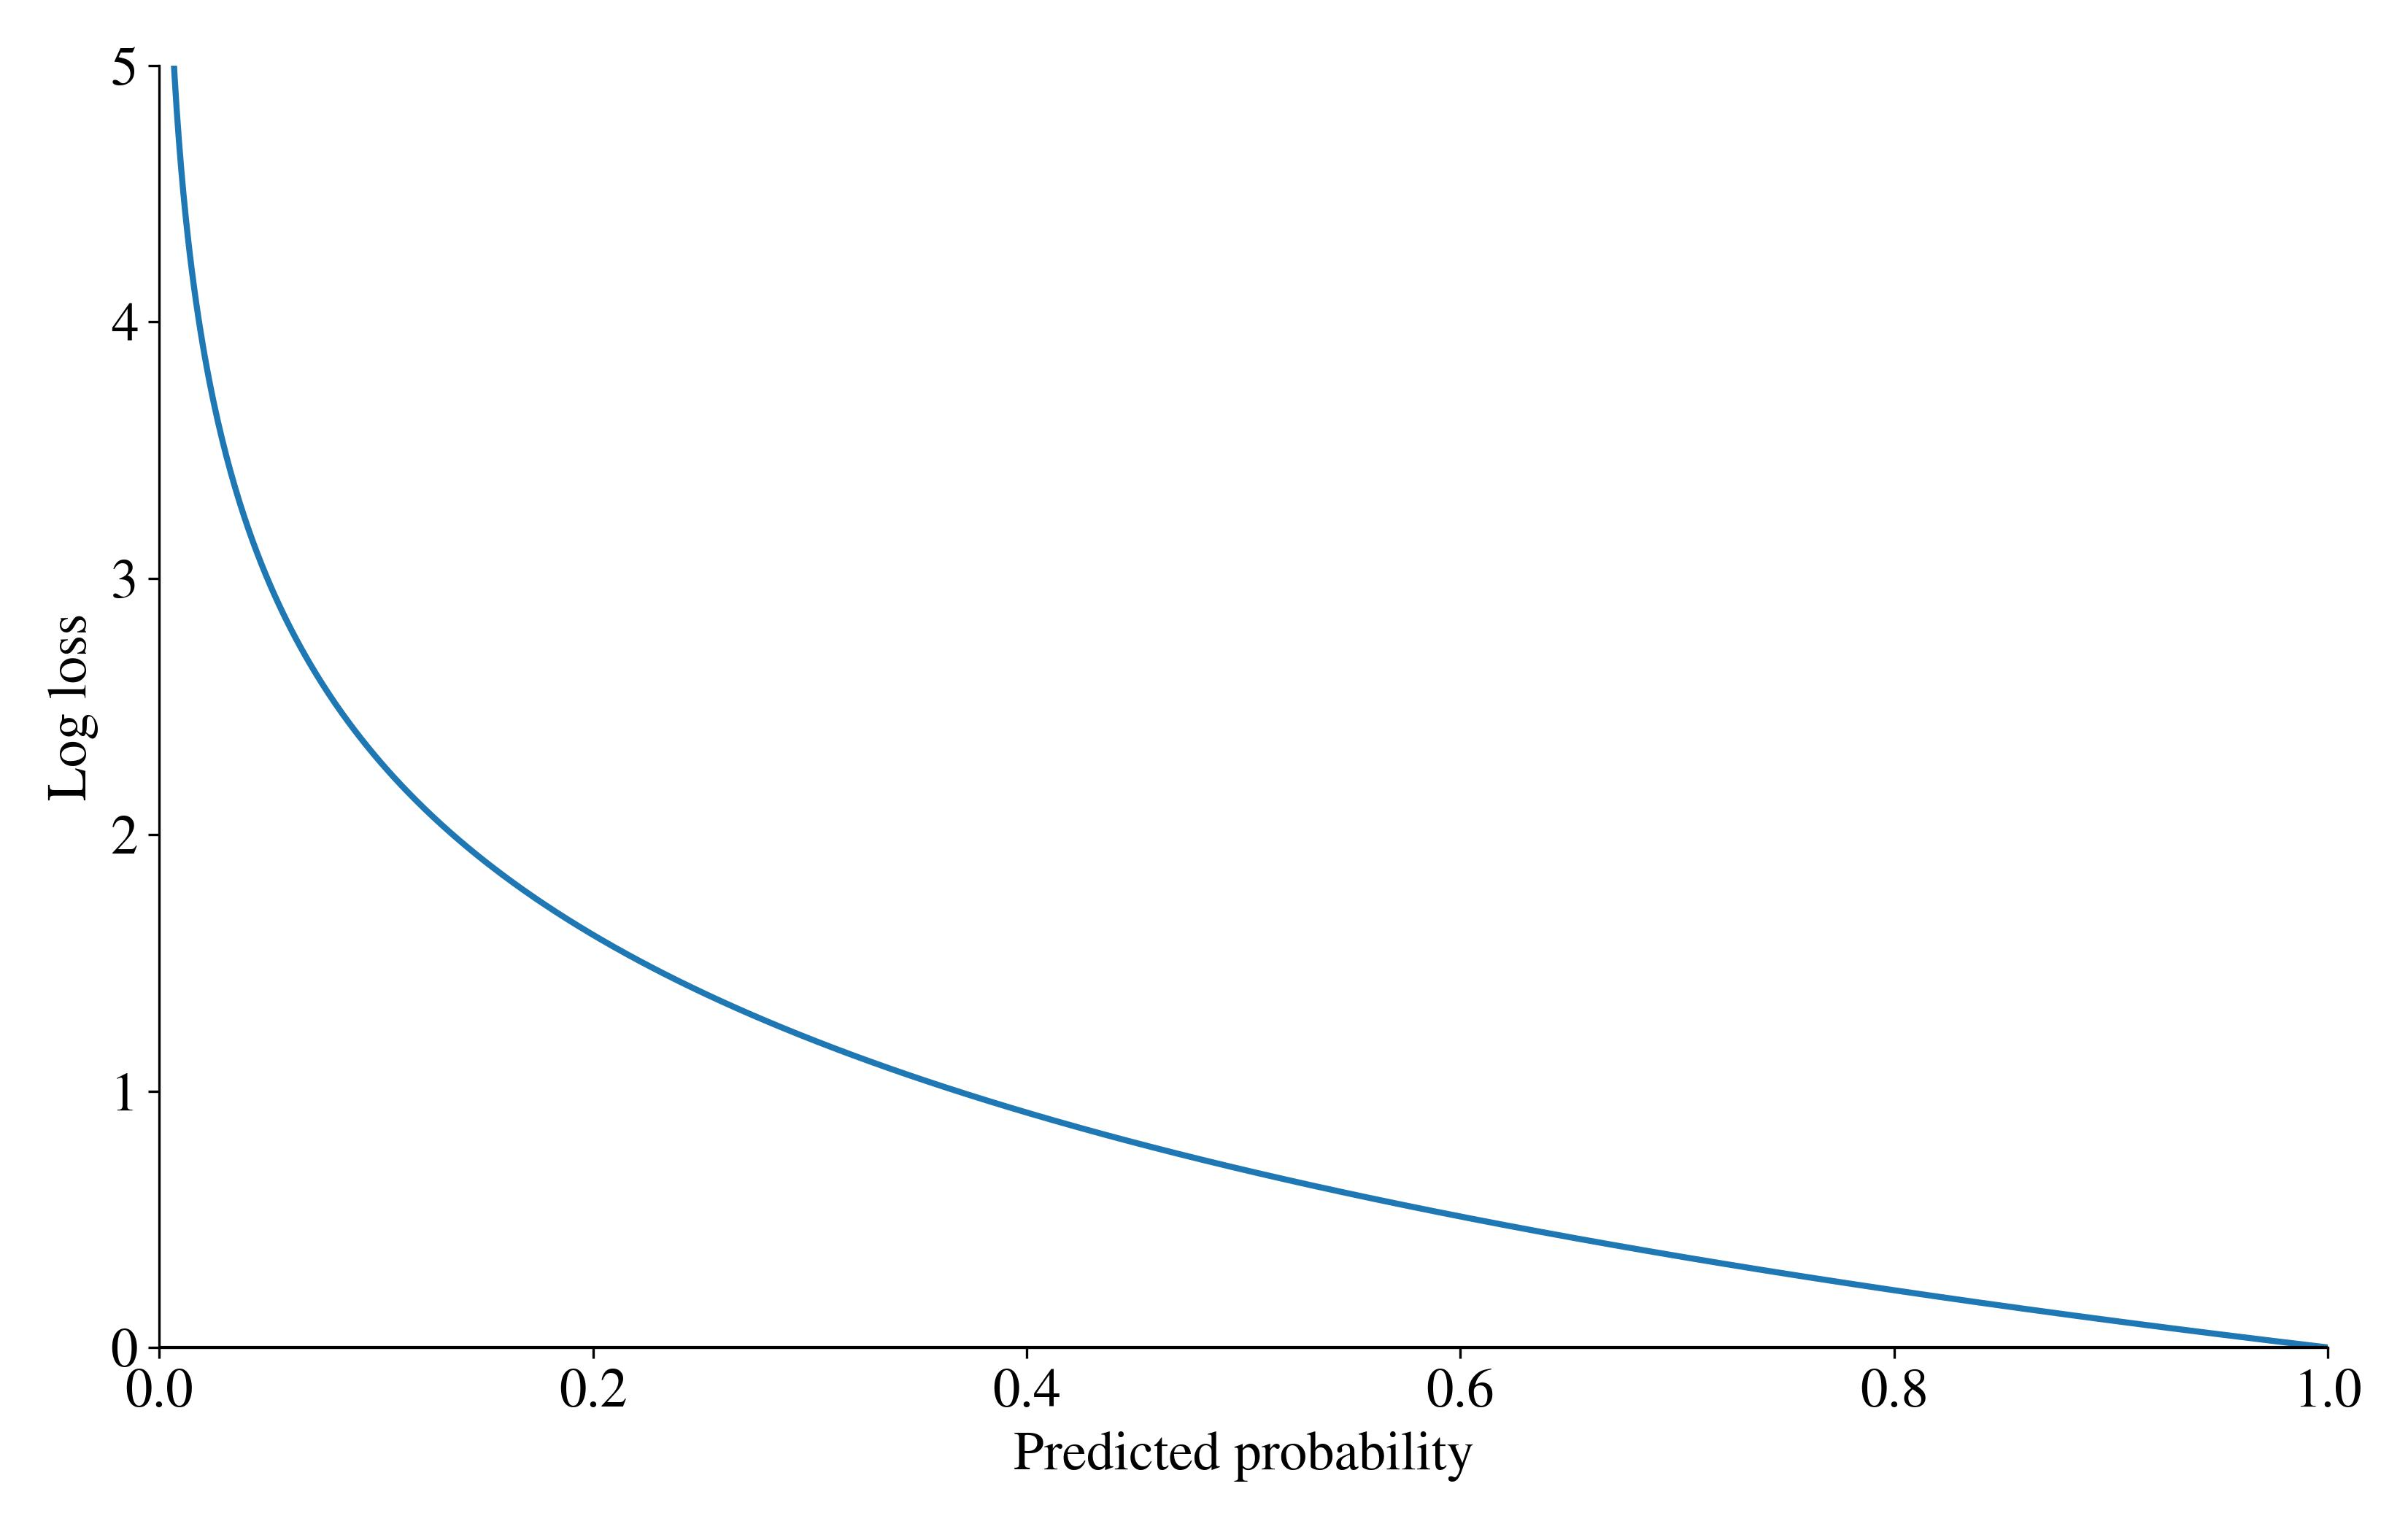
\includegraphics[width=130mm]{Figures/logloss.jpg}
    \centering{\begin{source}Author's simulation in Python\end{source}}\vspace{-1em}
\end{figure}



\section{ADASYN Oversampling}
\label{sec:adasyntheory}
Since this thesis pertains to the data set of defaulted loans, which target variable distribution is heavily skewed, it is needed to emphasize the imbalanced class issue, i.e., the class is strongly imbalanced as the frequency distribution of the majority class is significantly higher than the frequency distribution of the minority class. In case of defaulted loans, the majority class would be non--default status and the minority class would be default status.
This can cause serious degradation in model's performance as most of the models assume well--balanced class distributions, hence such models would be biased towards the majority class and would not be able to predict the minority class accurately \citep{prati2009data}.

To overcome this issue, one would use Random Undersampling or Random Oversampling to deal with the class imbalanced issue. The former randomly eliminates majority class instances whereas the latter randomly duplicates minority class instances.
However, both have particular drawbacks, as the random under-sampling may lead to a a significant loss of information, and random oversampling is lead to the high degree of repetation of minority instances. Both then could lead to model's overfitting and detoriation in model's performance \citep{ma2013imbalanced}.
This might be a significant issue when the target variable distribution is heavily imbalanced - assume that we have a data set of 1,000 instances where 990 instances belongs to majority class and 10 instances to minority class.
If we perform random undersampling in order to balance the target variable distribution, we would have to remove 980 instances and end up with undersampled data set of 20 instances, which is not acceptable for model training.
On the other hand, if we perform random oversampling, we would end up with 1,980 instances, where 980 instances would be the same as in the original data set, which would lead to the model's overfitting.

Therefore, the Adaptive Synthetic Sampling (henceforth ADASYN) technique is used for oversampling the minority class in this thesis.
ADASYN generates synthetic instances of the minority class based on the nearest neighbors of the minority class instances.
Such approach is more effective than Synthetic Minority Oversampling Technique (henceforth SMOTE) which also uses nearest neighbors to generate synthetic instances of minority class, however, ADASYN generates more synthetic instances which are hard--to--learn by K-Nearest Neighbors given the density distributtions, whereby SMOTE generates synthetic instances uniformly for each minority class instance.
 \citep{adasynhaibo}. 

In other words, ADASYN generates more synthetic instances in regions where the density of the majority class within $K$ nearest neighbors of minority instance is higher and fewer synthetic instances in regions where the density is lower, thereby ADASYN focuses on generating more hard--to--learn minority instances.
Thereby, it makes easier for the machine learning model to learn the decision boundary between the minority and majority classes and boost the model's performance by focusing on hard--to--learn instances \citep{adasynhaibo}.

Before oversampling algorithm's execution, first we need to calculate the number of instances of minority class to be synthetically generated in order to balance the target variable distribution. The number of instances to be generated $G$ is calculated as follows:
\begin{equation}\label{eq}
    G = \left(m_{l} - m_{s}\right) \times \beta
\end{equation}
where $m_l$ is the number of majority class instances, $m_s$ is the number of minority class instances and $\beta$ indicates the desired ratio between the numbers of majority and minority class instances after oversampling.

Then, for each minority class instance $x_i$, using $K$-Nearest Neighbors with Euclidean distance calculate the ratio $r_i$ as:
\begin{equation}\label{eq}
   r_{i} = \frac{\delta_{i}} {K}
\end{equation}
where $\delta_{i}$ is the number of majority class instances within the $K$ nearest neighbors of $x_i$.
In such case, higher $r_i$ indicates dominance of the majority class in given specific neighborhood of $x_i$ \citep{nian2018introduction}.
Subsequently, all the $r_i$ ratios are normalized as:
\begin{equation}\label{eq}
    \hat{r}_{i} = \frac{r{i}}{\displaystyle\sum_{i=1}^{m_{s}} r_{i}}
\end{equation}
In such way that sum of all the normalized $\hat{r}_i$ ratios is equal to 1. Hence, we can denote $\hat{r}_i$ as the density distribution.
\begin{equation}\label{eq}
    \sum_{i=1}^{m_{s}} \hat{r}_{i} = 1
\end{equation}

Finally, the oversampling process is initialized.
For each minority class instance $x_i$, calculate the number of instances to be synthetically generated based on the respective density distribution $\hat{r}_i$ and the total number of instances to be synthetically generated $G$. Thus, for the minority classes with higher density, it generates more synthetic instances, since those instances are hard--to--classify by the K-Nearest Neighbors.
\begin{equation}\label{eq}
    G_i = G \times \hat{r}_{i}
\end{equation}
Further, for each minority class instance $x$, generate $G_i$ synthetic instances $s_i$ as follows:
\begin{equation}\label{eq}
    s_i = x_i + \left(x_{zi} - x_{i} \right) \times \lambda
\end{equation}
where $x_{zi}$ represents the radnomly chosen minority class instance within the $K$ nearest neares neighbors for $x_i$, and $\lambda \in \left[0,1\right]$ is a random number.

\newpage
\section{Optimal Binning}
\label{sec:optbinningtheory}
In the context of data preprocessing, it is crucial to consider the most appropriate feature transformation method that optimizes the performance of machine learning models.
Although common approaches such as dummy encoding, standardization, logarithmic transformation, and normalization are widely used, they may not always be suitable for a given data set due to the presence of certain characteristics.
For instance, dummy encoding (also known as one--hot encoding) may not be suitable for categorical features with a large number of categories as it could lead to the curse of dimensionality, therefore, it may result in the decrease of model's performance \citep{bera2021dimensionality}.
Standardization may not be appropriate for features with a large number of outliers as it may result in a loss of information.

Therefore, alternative approaches such as discretization or binning are increasingly being used. Binning is a categorization process to transform a continuous variable into a small set of groups or bins \citep{zeng2014necessary}. This approach enables the identification of outliers within bins and reduce their impact, and additionally, it can capture missing values without requiring the removal or imputation of such values.

In this thesis, we employ the \lstinline{BinningProcess} from the \lstinline{optbinning} module in Python for an optimal binning of both numeric and categorical features with respect to the target variable, developed by Guillermo Navas--Palencia \citep{navas2020optimal}. 
This approach involves grouping the values of a continuous variable into discrete intervals, or "bins", based on their relationship with the target variable.
Similarly, for categorical features, the approach involves grouping the categories based on their relationship with the target variable.
In general, the optimal binning is solved by iteratively merging an initial granular discretization until imposed constraints are satisfied. Particularly, the optimal binning process consists of two phases - pre--binning process (for generating initial granular discretization) and subsequent optimization (for satisfying imposed constraints).
The former phase usually uses decision tree to generate initial split points to create pre--bins which are further merged while maximizing Information Value (also known as Jeffreys' divergence) while accounting for the constraints. As Navas--Palencia states \citep{navas2020optimal}, Such constraints are:
\begin{itemize}\setlength\itemsep{0em} 
    \item \textbf{Creation of separate bins for missing values:} Since missing values can have a significant impact on the target variable, hence is important to create a separate bin for them.
    \item \textbf{Minimum bin size constraint:} At least 5 \% of the total number of instances should be observed within given bin. Such constraint ensures a bin's representativness.
    \item \textbf{Each bin should have at least one instance of each target class:} Application of such constraint allows to compute divergence measure.
\end{itemize}
Thus, using the optimal binning process, the goal is the maximize discriminatory power among bins, i.e., divergence measure.
For more information about optimal binning, please refer to \citep{navas2020optimal}.

After the binning process, the bins as categorical values need to be encoded into numeric values. The most common approach in credit risk modelling is Weight--of--Evidence (henceforth WoE) encoding. The WoE is a commonly used measure of the strength of association between a binary target variable and an independent variable.
According to Witzany \citep{witzany2017credit}, the WoE of categorical value $c$ can be expressed as the change between the overal log odds ratio and the log odds ratio given the value $c$, hence:
\begin{equation}\label{eq}
    WoE\left(c\right) = \ln\left(\operatorname{Pr}\left(c \mid Y = 0 \right) \right) - \ln\left(\operatorname{Pr}\left(c \mid Y = 1 \right) \right)
\end{equation}
Assuming feature $X$ and its respective bin $b_i$, thus $b_i \in X$, we can express WoE in terms of $b$ as follows:
\begin{equation}\label{eq}
    WoE_{X, b}= \ln \left(\frac{\Pr{\left(X = b\;\middle|\;Y = 0\right)}}{\Pr{\left(X = b\;\middle|\;Y = 1\right)}}\right)
\end{equation}
According to Navas--Palencia \citep{navas2020optimal}, the WoE for bin $i$ can be also computed as:
\begin{equation}\label{eq}
    WoE_{i} = \ln \left( \frac{r^{ND}_i / r^{ND}_T} {r^{D}_i / r^{D}_T}  \right)
\end{equation}
where $r^{ND}_i$ is the number of non--default instances in given bin $i$, $r^{D}_i$ is the number of default instances in the given bin $i$, $r^{ND}_T$ is the total number of non--default instances in whole sample and $r^{D}_T$ is the total number of default instances in whole sample.
Thus, positive WoE value is indicates larger distribution of non--defaults, i.e. higher likelihood of non--default, while negative WoE value indicates larger distribution of defaults, i.e., higher likelihood of default.

\section{Hyperparameter Bayesian Optimization}
\label{sec:bayesoptheory}
Most of the machine learning models are configured by a set of hyperparameters which are not learned during the training process but need to be set beforehand. Such hyperparameters' values must be carefully chosen and considerably impact model's performance \citep{bischl2023hyperparameter}.
It is needed to point that the difference between parameter and hyperparameter - while paramater value is learnt during the training process from the data, on the other hand, hyperparameter value is set before the training process and cannot be learnt from the data \citep{owen2022hyperparameter}. In case of logistic regression, the parameters are estimated coefficients and intercept, while the hyperparameters are for instance regularization parameter, optimization solver etc.

Thus, it is recommended to select optimal hyperparameter values instead of relying on default hyperparameters.
Nonetheless, selecting optimal hyperparameter values can be very challenging, especially when there are many hyperparameters to tune.
Fortunately, in machine learning practice already exist several methods how to choose the best hyperparameters' values. The most common ones are Grid Search and Random Search.
The former approach tries all the possible combinations of hyperparameters' values from predetermined hyperparameter space, which can be very computationally expensive, when the number of hyperparameters is large \citep{marinov2019hyperparameter}, when the space of hyperparameter's values is too wide or when the data set is too large.
Regarding the latter approach, instead of trying al the possible combinations from the grid, it randomly selects samples of hyperparameters combinations. Although such approach can be less computationally expensive, it does not guarantee to find the global optimum.
Another issue pertaining to both approach is that they do not consider any information from previous iterations and rather check all possible hyperparameter combinations or randomly select hyperparameter combinations, respectively.

The compromise for such drawbacks is hyperparameter tuning with Bayesian Optimization, which is able to find the best hyperparameters' values in less time and with less computational resources than Grid Search and also, it leads to better model's performance than Random Search despite the longer optimization time \citep{drahokoupil2022application}.
Bayesian Optimization is a hyperparameter tuning method which uses infromation from previous iterations in order to make more informed decsion about which hyperparameters' values to try next.
The main property of hyperparameter tuning is the objective function which we want to optimize (i.e., maximize or minimize in case of a score and loss, respectively), which input is the hyperparameters' values and the output is the score or loss. However, the objective function is not known beforehand and is very computionally expensive to evaluate.


Therefore, Bayesian Optimization uses a surrogate function which is the approximation and probability representation of the objective function. The most common surrogate function is the Gaussian Process (henceforth GP) which is able to produce accurate approximations as well as the uncertainty around the approximations \citep{wang2020bayesian}.
According to Owen \citep{owen2022hyperparameter}, GP is utilized as the prior for the objective function along the posterior, which we want to update.
In other words, the prior captures the initial belief about the objective function, while the posterior is the updated distribution combining the prior belief and the observed evaluations of the objective function, i.e., it reflects the current belief about the objective function, hence the relation between the hyperparameters' values and the score or loss.
GP is the generalization of the normal distribution and describes the distribution over functions (not the distribution of a random variable), hence the objective function $f$ follows a normal distribution with noise as:
\begin{equation}\label{eq}
    y = f\left(x\right) + \epsilon
\end{equation}
Let us denote $f_{1:n} = \{ f\left(x_1\right), f\left(x_2\right), \ldots, f\left(x_n\right)\}$ as a set of $n$ observations of the objective function, where $m\left(x_{1:n}\right)$ is the mean function and $K$ is the covariance kernel. Hence, such set follows normal distribution as well:
\begin{equation}\label{eq}
    f_{1:n} \sim N\left(m\left(x_{i:n}\right), K\right)
\end{equation}
Henceforth, the distribution of prediction generated by GP also follows normal distribution as:
\begin{equation}\label{eq}
    p\left(y \mid x, D\right) \mid N\left(y \mid \mu^{*}, \sigma^{*2}\right)
\end{equation}
where $\mu^{*}$ and $\sigma^{*2}$ can by analytically derived from the $K$ kernel, and $D$ represents observed data regarding the previously evaluated iterations of hyperparameters' values.

Furthermore, Bayesian Optimization also employs acquisition function which accounts for which set of hyperparameters should be used in the next iteration \citep{owen2022hyperparameter}. Particularly, the next hyperparameters' set is chosen based on the location where the acquisition function is maximized.
The most common acquisition function is the Expected Improvement (henceforth EI), which is according to Owen \citep{owen2022hyperparameter} defined as follows assuming that $ \sigma\left(x\right) \neq 0$:
\begin{equation}\label{eq}
    EI(x) = \left(\mu\left(x\right) - f\left(x^{+}\right)\right) \times \Phi\left(Z\right) + \sigma\left(x\right) \times \phi\left(Z\right)
\end{equation}
where $\sigma\left(x\right)$ is the uncertainty, $\mu\left(x\right)$ is the expected performance which are both captured by surrogate model. $f\left(x^{+}\right)$ indicates the current best value of the objective function, $\Phi\left(Z\right)$ and $\phi\left(Z\right)$ are the cumulative distribution function and probability density function of the standard normal distribution, respectively.
Moreover, EI allows to balance between exploration and exploitation, where the former refers to the searching for the uknown regions where the objective function may have higher values, i.e, the hyperparameters' values which have not been evaluated yet, while the latter refers to the searching near the best observed values of the objective function, i.e.,near by the hyperparameters' values which have been evaluated already.
Referring to Owen \citep{owen2022hyperparameter}, higher expected performance $\mu\left(x\right)$ compared to the current best value $f\left(x^{+}\right)$ will favor the exploitation process, whereby a very high uncertainty $\sigma\left(x\right)$ will support exploration process.

\section{Forward Sequential Feature Selection}
\label{sec:fsfstheory}
Instead of using all the features in data set, we use only the subset of the most relevant ones, which can further reduce the dimensionality of data set, boost model performance, save computational resources and reduce overfitting. Such process is called feature selection and can be defined as the process of detecting the most relevant features and discarding the noisy redundant ones. \citep{bolon2015feature}.

With respect to the target variable, we distinguish 2 most common types of feature selection approaches: (1) filter methods and (2) warapper methods.
Using the former approach, the feature selection is independent on a machine learning model itself, but rather is performed using univariate statistical tests, such as correlation measures, Chi--square test, Fisher score and others \citep{kaushik2016introduction}, and chooses those ones with the highest or lowest values.
This approach is used when we prefer lower computational cost and faster feature selection process, but since it does no take into account the model itself, it does not have to able to select the features which would be optimal for particular model.
Regarding the latter approach, the feature selection is based on a specific machine learning model and follows a greedy search approach by evaluating all the possible combinations of features against the evaluation metric criteria \citep{Verma2020}. Although, such approach is very computationally expensive, it is able to select the optimal features for a particular model.

The most common wrapper method for feature selection is Recursive Feature Elimination (henceforth RFE). Such method takes a machine learning model as an base estimator, fit the model on whole set of features, computes and ranks their coefficients or feature importances, eliminates the least important features and repeats the process until the desired number of features is reached \citep{Brownlee2020} or until the stop criteria is met.
However, the drawback of RFE is that it always requires feature importances or coefficients to compute, which is not suitable for models which do not produce any coefficients nor feature importances, such as KNN or Naive Bayes. Therefore, this approach is not implemented in this thesis.

Instead, the feature selection is performed with Sequential Feature Selection (henceforth SFS). Such method is iteratively adding (or removes) features the set sequentially. Hence, there are two approaches, Forward SFS and Backward SFS.
The former approach keeps adding features to the set until the desired number of features is reached, while the latter approach starts with the whole set of features and removes them until the desired number of features is reached.
In this thesis, Forward SFS is used since it was way more computationally efficient than Backward SFS within author's analysis. In particular, Forward SFS starts with an empty set of features and afterwards, variant features are sequentially added until the desired number of features is reached  or until the addition of extra features does not reduce the criterion \citep{Verma2021}. 
According to Scikit-learn's documentation \citep{sfs}, at each stage, SFS chooses the best feature to add based on the cross--validation score. 